\documentclass[11pt, a4paper]{book}
\usepackage{amsmath, amssymb, amsbsy}
\usepackage[amsmath, thmmarks]{ntheorem}
\usepackage{algorithm}
\usepackage{algpseudocode}
\usepackage{xcolor}
\usepackage{tikz}
\usepackage{paralist}
\usepackage{nicefrac}
\usepackage{minted}
\usepackage[colorlinks]{hyperref}
% =========== 


% ============================= Pseudocode Customization =======================
% Packages: algorithm, algpseudocode.
\algrenewcommand{\algorithmicrequire}{\textbf{Input:}}
\algrenewcommand{\algorithmicensure}{\textbf{Output:}}
\algnewcommand\algorithmicto{\textbf{to} } % a trailing space is needed.
\algnewcommand\algorithmicbreak{\textbf{break}} % break keyword.
\newcommand{\breakif}[1]{\State \textbf{if} {#1} \textbf{then break}}


% ============================= Math Theorem Envs ==============================
\theorembodyfont{\normalfont}
\newtheorem{df}{Definition}[section]
\newtheorem{thm}[df]{Theorem}
\newtheorem{eg}[df]{Example}
\newtheorem{prop}[df]{Proposition}
\newtheorem{lem}[df]{Lemma}
\newtheorem{cor}[df]{Corollary}
\newtheorem{re}[df]{Remark}

% Customize proof env.
\theoremstyle{nonumberplain} % no numbering
\theoremsymbol{$\square$}    % proof end with square.
\newtheorem{pf}{Proof}


% =============================== Operators ====================================
\DeclareMathOperator{\ent}{Entropy}
\DeclareMathOperator*{\p}{\mathbb{P}} % probability.
\DeclareMathOperator{\sign}{sign}
\DeclareMathOperator*{\argmax}{argmax}
\DeclareMathOperator*{\argmin}{argmin}
\DeclareMathOperator*{\E}{\mathbb{E}} % Expectation.
\DeclareMathOperator{\dist}{dist} % distance.
\DeclareMathOperator{\indi}{\mathbb{I}}
\DeclareMathOperator{\tr}{tr} % trace of an matrix.


% =============================== New Commands =================================
% Logical connectives:
\newcommand{\OR}{\textbf{OR} } % a space is needed here.
\newcommand{\AND}{\textbf{AND} } 
\newcommand{\XOR}{\textbf{XOR} } 

% Math commands:
\newcommand{\T}[1]{\ensuremath{{#1}^\mathsf{T}}} % Matrix transposition.
\newcommand{\inv}[1]{\ensuremath{{#1}^{-1}}} % Inversion.
\newcommand{\V}[1]{\ensuremath{\boldsymbol{#1}}}

% Shorthand commands:
\newcommand{\hypo}[1]{\ensuremath{{#1}: \mathcal{X} \longrightarrow \mathcal{Y}}} % Hypothesis function.
\newcommand{\dataset}{\ensuremath{D = \{(\V{x}_1, y_1), \ldots, (\V{x}_m, y_m)\}}} % Labeled training set.
\newcommand{\st}{\text{s.t.\ }}
\newcommand{\magenta}[1]{\textcolor{magenta}{#1}} % turn the color of text into magenta.
\newcommand{\hl}[2][yellow]{\colorbox{#1}{#2}} % highlight the text.
\newcommand{\pfrac}[2]{\ensuremath{\frac{\partial {#1}}{\partial {#2}}}}

% =====================================================
\numberwithin{equation}{section}

% =============================Python Code Customization========================
% Package: minted
\setminted[python]{frame=single, linenos=true, numbersep=3pt, autogobble=true, mathescape=true}

% =============================== Document =====================================
\begin{document}

% ========Title Page====================
\title{\textbf{Machine Learning Notes}}
\author{DeepWalter\thanks{Email: deepwalter.cn@gmail.com}}
\date{}
\maketitle

\frontmatter

% ========Table of Contents=============
\tableofcontents

% ========
\mainmatter

% ========Part One: Basics===========================
\part{Basics}
% ========Model Assessment and Selection======
\chapter{Model Assessment and Selection}
\section{Empirical Error and Overfitting}

\section{Assessment}

\section{Performance Measurement}
\subsection{Error Rate and Accuracy}
Error rate is the most direct measurement of performance. It is defined as the ratio of misclassified examples,
i.e.
$$err(f; D) = \frac{1}{m} \sum_{i=1}^m \mathbb{I}(f(\V{x}_i) \neq y_i)$$
where $m$ is the total number of examples. The accuracy is just the complement of error rate:
$$acc(f; D) = 1 - err(f; D)$$
Generally, for a distribution $\mathcal{D}$ over a data set $D$ with pdf (pmf) $p$, the error rate is defined as
\begin{equation}
    err(f;\mathcal{D}) = \int_{\V{x} \sim \mathcal{D}}\mathbb{I}(f(\V{x}) \neq y) p(\V{x})\diff{\V{x}}
\end{equation}

\subsection{Precision, Recall and F1 Score}
% Confusion matrix of classification.
\begin{table}[ht]
\begin{center}
    \begin{tabular}{|c|c|c|}\hline
        \diagbox{Fact}{Prediction} & Positive & Negative\\
        \hline
        True & TP & FN\\
        \hline
        False & FP & TN\\
        \hline
    \end{tabular}
\end{center}
\caption{Confusion Matrix}
\end{table}

Let $T$ and $F$ be the number of \textbf{true} and \textbf{false} examples respectively. Let $P$ and $N$ be
the number of \textbf{positive} and \textbf{negative} examples respectively. Then we have $m = P + N = T + F$
where $m$ is the number of total examples, and\marginnote{Look at the columns of the\\ confusion matrix.}
\begin{equation}
    \begin{cases}
        P &= TP + FP\\
        N &= FN + TN
    \end{cases}
\end{equation}
and\marginnote{Look at the rows of the\\ confusion matrix.}
\begin{equation}
    \begin{cases}
        T &= TP + FN\\
        F &= FP + TN
    \end{cases}
\end{equation}
The \textbf{precision} is defined as\marginnote{Of those positive examples, how many are truly positive? }
\begin{equation}
    p = \frac{TP}{P} = \frac{TP}{TP + FP}
\end{equation}
The \textbf{recall} is defined as\marginnote{How many truly positive \\examples have been picked out?}
\begin{equation}
    r = \frac{TP}{T} = \frac{TP}{TP + FN}
\end{equation}

% precision-recall curve.
\begin{figure}[ht]
    \begin{center}
    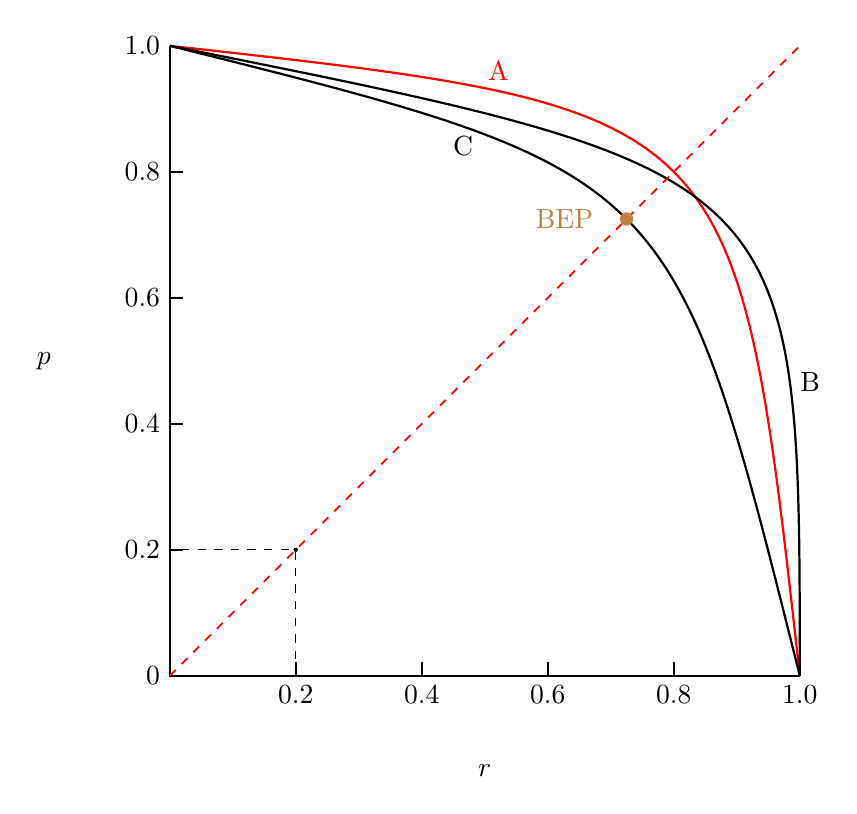
\begin{tikzpicture}[scale=8]
        \draw [thick] (0, 1) -- (0, 0) -- (1, 0);
        % \draw [thick] (0, 1) to [out=-30, in=110] (1, 0);
        % \draw [thick] (0, 1) to [out=-10, in=90] (1, 0);
        % \draw [thick, red] (0, 1) to [out=0, in=105] (1, 0);
        \draw [red, thick] (0, 1) .. controls (0.9, 0.9) .. (1, 0) node[above, near start] {A};
        \draw [thick] (0, 1) .. controls (1.0, 0.8) .. (1, 0) node[right, near end] {B};
        \draw [thick] (0, 1) .. controls (0.8, 0.8) .. (1, 0) node[below, near start] {C};
        \draw [semithick, red, domain=0:1, dashed] plot (\x, \x);
        \draw[dashed] (0.2, 0) -- (0.2, 0.2) -- (0, 0.2);

        \foreach \x in {0.2, 0.4, 0.6, 0.8} {
            \draw (\x, 0) node[below] {$\x$} [thick] -- ++(0, 0.6pt);
            \draw (0, \x) node[left] {$\x$} [thick] -- ++(0.6pt, 0);
        }
        \node [left] at (0, 0) {$0$};
        \node [below] at (1, 0) {$1.0$};
        \node [left] at (0, 1) {$1.0$};
        \node at (0.5, -0.15) {$r$};
        \node at (-0.2, 0.5) {$p$};
        % \draw [fill=magenta] (0.725, 0.725) circle [radius=0.01];
        % \node [left] at (0.725, 0.725) {BEP};
        \fill [brown] (0.725, 0.725) circle (0.3pt) node[left=0.3cm] {BEP};
        \fill (0.2, 0.2) circle (0.1pt);
    \end{tikzpicture}
    \end{center}
    \caption{Precision-Recall Curve}\label{pr_curve}
\end{figure}
In many algorithms, for example the logistic regression, we first compute a value from the given feature
vector of an example, then we compare it
with a threshold value to determine whether it is positive or negative. In order to get high recall, we can
mark all examples as positive (that is, set the threshold value to a very small value), which makes $FN = 0$;
but this will make the precision low since all false examples are classified as positive too.
Similarly, in order to achieve high precision, we can set the threshold value large (that is, we only classify
an example as positive if we are confident enough), but this will leave many examples as negative, hence $FN$
is large, which causes low recall. In general, precision and recall can not both increase at the same time.
See figure~\ref{pr_curve}.\marginnote{For example, B performs better than C in figure~\ref{pr_curve}.} If one
learner's P-R curve is enclosed  by anothers', then the latter has a better performance. In other situations,
can use the \textbf{B}reak \textbf{E}vent \textbf{P}oint to compare two learners' performance. Here, the BEP
is just the point where precision equals recall. See figure~\ref{pr_curve} for an example.

The F1 score is defined as
\begin{equation}
    F1 = \frac{2}{\frac{1}{p} + \frac{1}{r}} = \frac{2pr}{p + r}
\end{equation}


\subsection{ROC and AUC}

\textbf{True/False Positive Rate} is defined as
\begin{equation}
    \begin{cases}
        TPR &= \dfrac{TP}{T} = \dfrac{TP}{TP + FN}\vspace{5pt}\\
        FPR &= \dfrac{FP}{F} = \dfrac{FP}{FP + TN}
    \end{cases}
\end{equation}
The \textbf{R}eceiver \textbf{O}perating \textbf{C}haracteristic curve uses true positive rate as vertical
axis and false positive rate as horizontal axis. Below is a ROC curve and the gray area is the
corresponding \textbf{A}era \textbf{U}nder \textbf{C}urve.
% ROC curve and AUC.
\begin{figure}[ht]
    \begin{center}
    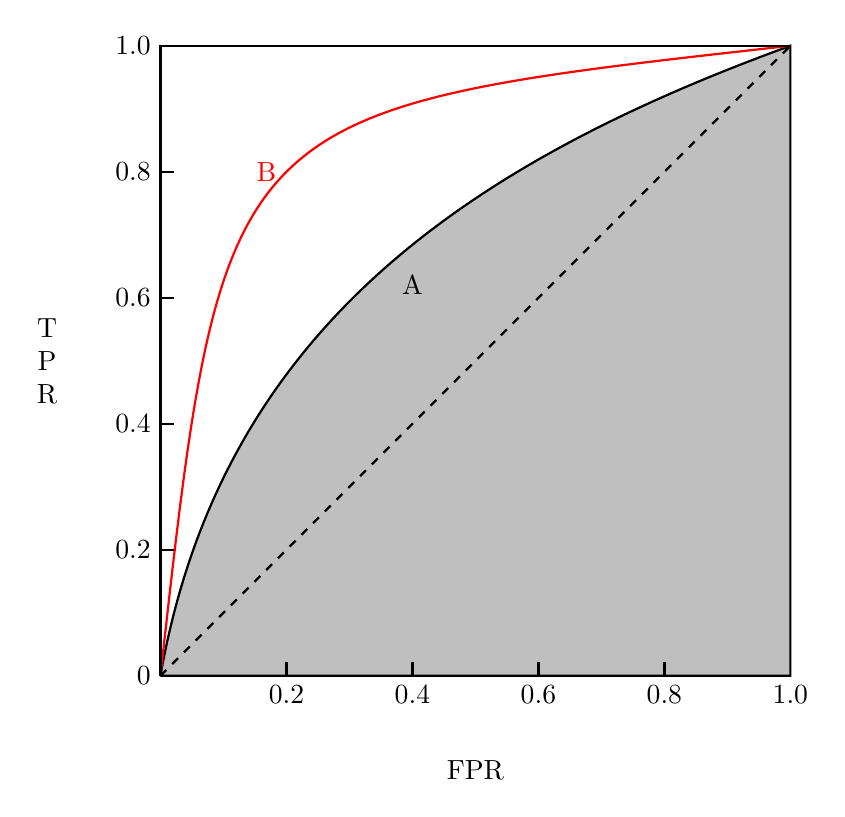
\begin{tikzpicture}[scale=8]
        \draw[thick, fill=lightgray] (0, 0) to [out=80, in=200] (1, 1) -- (1, 0) -- (0, 0);
        \draw[thick, red] (0, 0) .. controls (0.1, 0.9) .. (1, 1) node[left, midway]{B};
        \draw[dashed, thick] (0, 0) -- (1, 1);
        \draw[thick] (0, 0) -- (0, 1) -- (1, 1);

        \foreach \x in {0.2, 0.4, 0.6, 0.8} {
            \draw (\x, 0) node[below] {$\x$} [thick] -- ++(0, 0.6pt);
            \draw (0, \x) node[left] {$\x$} [thick] -- ++(0.6pt, 0);
        }
        \node [left] at (0, 0) {$0$};
        \node [below] at (1, 0) {$1.0$};
        \node [left] at (0, 1) {$1.0$};
        \node [below] at (0.4, 0.65) {A};
        \node at (0.5, -0.15) {FPR};
        \node [align=center] at (-0.18, 0.5) {T\\P\\R};
        \end{tikzpicture}
    \end{center}
    \caption{ROC Curve}\label{ROC}
\end{figure}

When $TPR = FPR$, we have
$$\frac{TP}{T} = \frac{FP}{F}$$
Notice that $T = TP + FN$ and $F = FP + TN$, we have
$$\frac{FN}{T} = \frac{TN}{F}$$
That is, for any example, we predict it to be positive with a given probability. So in figure~\ref{ROC}, the
dashed diagonal corresponds to the random guess model (with a fixed probability). When $(FPR, TPR) = (1, 0)$,
we have
\begin{equation*}
    \begin{cases}
        TP &= 0\\
        TN &= 0
    \end{cases}
\end{equation*}
that is, $acc = 0$. When $(FPR, TPR) = (0, 1)$, we have
\begin{equation*}
    \begin{cases}
        FP &= 0\\
        FN &= 0
    \end{cases}
\end{equation*}
that is, $acc = 1$. When $(FPR, TPR) = (0, 0)$, we have
\begin{equation*}
    \begin{cases}
        FP &= 0\\
        TP &= 0
    \end{cases}
\end{equation*}
that is, the predictor marks all examples as negative. When $(FPR, TPR) = (1, 1)$, we have
\begin{equation*}
    \begin{cases}
        FN &= 0\\
        TN &= 0
    \end{cases}
\end{equation*}
that is, the predictor marks all example as positive.

Of course, if a learner's ROC is fully enclosed by anothers', then the latter has a better performance.
For example, in figure~\ref{ROC}, the learner with ROC B performs better than the one with ROC A.
If two learners' ROCs cross with each other, then we may compare their AUCs and again we prefer the one with
larger AUC\@.

\section{Bias and Variance}

Let's consider the bias and variance decomposition of supervised learning. Asssume $\mathcal{X}$ is the
instance space and $\mathcal{Y}$ the label space. Let $\p$ be the joint distribution over
$\mathcal{X} \times \mathcal{Y}$ and $p$ the joint pdf. Let \dataset\ be any \iid dataset \wrt the
distribution $\p$, that is $D \sim \p^m$. For any given instance \V{x}, we have

\begin{df}[Expected label]
    The expected label of \V{x} is defined as:
    \begin{equation}
        \bar{y}(\V{x}) := \E_{y|\V{x}}[y] := \int_y y\,p(y|\V{x})dy
    \end{equation}
\end{df}

Notice that $\bar{y}(\V{x})$ is deterministic \wrt \V{x}, it is the true model that we want to approximate.
Naturally, the data-intrinsic noise is defined as:
\begin{equation}
    \E_{\V{x}, y}\left[{(\bar{y}(\V{x}) - y)}^2\right] = \int_{\V{x}} \int_y {(\bar{y}(x) - y)}^2 p(\V{x}, y)
    d\V{x}dy
\end{equation}
If we write the true model as $f(\V{x})$, then $y$ can be written as $y = f(\V{x}) + \varepsilon$ where
$\varepsilon$ is a random variable (for fixed \V{x}) \wrt $y$ \st $\E_{y}[\varepsilon] = 0$. If we assume that
$\varepsilon$ is independent of \V{x} and has variance $\sigma^2$, it is obvious from the above equation that
the data-intrinsic noise is just $\sigma^2$.

For any given algorithm $\mathcal{A}$, we can use it to train a learner $h_D = \mathcal{A}(D)$ from the
dataset $D$. Since $D$ is a random variable and $h_D$ is a function of $D$, $h_D$ is also a random variable.

\begin{df}[Expected learner]
    The expected learner given by the algorithm $\mathcal{A}$ on $m$ training examples is defined as:
    \begin{equation}
        \bar{h} := \E_{D \sim \p^m}[h_D] := \int_D h_D\, p(D) dD
    \end{equation}
\end{df}

\begin{df}[Variance]
    The variance of the learners given by the algorithm $\mathcal{A}$ on $m$ training examples is defined as:
    \begin{equation}
        \E_{\V{x}, D}\left[{(h_D(\V{x}) - \bar{h}(\V{x}))}^2\right]
    \end{equation}
\end{df}

\begin{df}[Bias]
    The bias of the algorithm $\mathcal{A}$ on $m$ training examples  is defined as the expected square error
    of the expected learner and the true model, i.e.
    \begin{equation}
        \E_{\V{x}}\left[{(\bar{h}(\V{x}) - \bar{y}(\V{x}))}^2\right]
    \end{equation}
\end{df}

For any given $h_D$, as usual we have

\begin{df}[Expected true error]
    The expected true error of a learner $h_D$ is defined as:
    \begin{equation}
        \E_{(\V{x}, y) \sim \p}\left[{(h_D(\V{x}) - y)}^2\right] = \int_{\V{x}} \int_y {(h_D(\V{x}) - y)}^2
        p(\V{x}, y) d\V{x} dy
    \end{equation}
\end{df}

Similar to the above expected true error \wrt to a specific learner, we can defined the expected true error
\wrt to an algorithm $\mathcal{A}$.

\begin{df}[Expected true error]
    The expected true error of an algorithm $\mathcal{A}$ is defined as:
    \begin{equation}
        \E_{\substack{(\V{x}, y) \sim \p \\ D \sim \p^m}}\left[{(h_D(\V{x}) - y)}^2\right] =
        \int_D \int_{\V{x}} \int_y {(h_D(\V{x}) - y)}^2 p(\V{x}, y) p(D) d\V{x} dy dD
    \end{equation}
\end{df}

In order to understand the expected true error of an algorithm, we can decompose it into three parts as
following:
\begin{align*}
    \E_{\V{x}, y, D}\left[{(h_D(\V{x}) - y)}^2\right] &= \E_{\V{x}, y, D} \left[{(h_D(\V{x}) - \bar{h}(\V{x})
    + \bar{h}(\V{x}) - y)}^2 \right] \\
    &= \E_{\V{x}, D} \left[{(h_D(\V{x}) - \bar{h}(\V{x}))}^2\right] +
    \E_{\V{x}, y}\left[{(\bar{h}(\V{x}) - y)}^2\right]\\
    &\quad\quad + 2\E_{\V{x}, y, D}\left[{(h_D(\V{x}) - \bar{h}(\V{x}))(\bar{h}(\V{x}) - y)}\right]\\
\end{align*}
Since
\begin{align*}
    \E_{\V{x}, y, D}\left[(h_D(\V{x}) - \bar{h}(\V{x}))(\bar{h}(\V{x}) - y)\right] &=
    \E_{\V{x}, y}\left[\E_D\left[(h_D(\V{x}) - \bar{h}(\V{x}))(\bar{h}(\V{x}) - y)\right]\right] \\
    &= \E_{\V{x}, y}\left[(\bar{h}(\V{x}) - y) \E_D\left[(h_D(\V{x}) - \bar{h}(\V{x}))\right]\right] \\
    &= 0
\end{align*}
we have:
\begin{equation}\label{bias-variance:1}
    \E_{\V{x}, y, D}\left[{(h_D(\V{x}) - y)}^2\right] = \E_{\V{x}, D} \left[{(h_D(\V{x}) -
    \bar{h}(\V{x}))}^2\right] + \E_{\V{x}, y}\left[{(\bar{h}(\V{x}) - y)}^2\right]
\end{equation}
Similarly,
\begin{align*}
    \E_{\V{x}, y}\left[{(\bar{h}(\V{x}) - y)}^2\right] &= \E_{\V{x}, y}\left[{(\bar{h}(\V{x}) - \bar{y}(\V{x})
    + \bar{y}(\V{x}) - y)}^2\right]\\
    &= \E_{\V{x}}\left[{(\bar{h}(\V{x}) - \bar{y}(\V{x}))}^2\right] +
    \E_{\V{x}, y}\left[{(\bar{y}(\V{x}) - y)}^2\right] \\
    &\quad\quad + 2\E_{\V{x}, y}\left[(\bar{h}(\V{x}) - \bar{y}(\V{x}))(\bar{y}(\V{x}) - y)\right]
\end{align*}
and
\begin{align*}
    \E_{\V{x}, y}\left[(\bar{h}(\V{x}) - \bar{y}(\V{x}))(\bar{y}(\V{x}) - y)\right] &=
    \E_{\V{x}}\left[\E_{y|\V{x}}\left[(\bar{h}(\V{x}) - \bar{y}(\V{x}))(\bar{y}(\V{x}) - y)\right]\right]\\
    &= \E_{\V{x}}\left[(\bar{h}(\V{x}) - \bar{y}(\V{x})) \E_{y|\V{x}}\left[(\bar{y}(\V{x}) - y)\right]\right]\\
    &= 0
\end{align*}
implies
\begin{equation}\label{bias-variance:2}
    \E_{\V{x}, y}\left[{(\bar{h}(\V{x}) - y)}^2\right] =
    \E_{\V{x}}\left[{(\bar{h}(\V{x}) - \bar{y}(\V{x}))}^2\right]
    + \E_{\V{x}, y}\left[{(\bar{y}(\V{x}) - y)}^2\right]
\end{equation}
Combine equation~\eqref{bias-variance:1} and~\eqref{bias-variance:2}, we have:
\begin{equation}\begin{split}
    \E_{\V{x}, y, D}\left[{(h_D(\V{x}) - y)}^2\right] &= \E_{\V{x}, D} \left[{(h_D(\V{x}) -
    \bar{h}(\V{x}))}^2\right] + \E_{\V{x}}\left[{(\bar{h}(\V{x}) - \bar{y}(\V{x}))}^2\right]\\
    &\quad\quad+ \E_{\V{x}, y}\left[{(\bar{y}(\V{x}) - y)}^2\right]
\end{split}\end{equation}
That is, the expected true error of an algorithm can be decomposed as the sum of the variance, the bias, and
the noise.

% ========Linear Models================
\chapter{Linear Model}
In a linear model, the learner takes the form of a (affine) linear function
$$y = \langle\V{w}, \V{x}\rangle + b = \langle\hat{\V{w}}, \hat{\V{x}}\rangle$$
where $\hat{\V{w}}=(\V{w}, b),\;\hat{\V{x}} = (\V{x}, 1)$.
\section{Linear Regression}

\section{Logistic Regression}

\section{Linear Discriminant Analysis}
The idea of linear discriminant analysis is to find a line with direction $\V{w}$ \st when
projected to this line, examples with the same label will stay close while examples with different
labels will be far away. When predicting, we first project the example onto the line, then assign it the
label of the group of examples which is closest to it.

Let \dataset\ be the data set, $\mathcal{Y} = \{0, 1\}$ the label space. Let\marginnote{$n_0 + n_1 = m$ and
$\V{\mu}_i$ is the center of examples with label $i$.} 
$X_i \in \mathbb{R}^{n_i \times n}$ be the matrix of all examples with label $i$ and 
$\V{\mu}_i \in \mathbb{R}^{1 \times n}$ the mean vector of all such examples. Let 
$$ \Sigma_i = \T{(X_i - \V{\mu}_i)}(X_i - \V{\mu}_i)$$
be the covariance matrix of all examples with label $i$. After
projecting onto the line $\V{w}$, $X_i$ becomes $X_i \T{\V{w}}$, and $\V{\mu}_i$ becomes
$\V{\mu}_i\T{\V{w}}$. Hence the covariance matrix becomes $\V{w} \Sigma_i \T{\V{w}}$, which is a real number.
To make examples with the same label stay close and examples with different labels stay away, we want small 
variances $\V{w} \Sigma_i \T{\V{w}}$ and a large distance $\norm{\V{\mu}_0\T{\V{w}} - \V{\mu}_1\T{\V{w}}}^2$.
That is, we want to maximize
\begin{equation}\label{lda_J}
    J = \frac{\norm{\V{\mu}_0\T{\V{w}} - \V{\mu}_1\T{\V{w}}}^2}{\V{w} \Sigma_0 \T{\V{w}} + 
    \V{w} \Sigma_1 \T{\V{w}}}
\end{equation}
If we define the \textbf{within-class scatter matrix} as
\begin{equation}
    S_w = \sum_{\V{x}\in X_0} \T{(\V{x} - \V{\mu}_0)}(\V{x} - \V{\mu}_0)
    + \sum_{\V{x}\in X_1} \T{(\V{x} - \V{\mu}_1)}(\V{x} - \V{\mu}_1)
\end{equation}
and \textbf{between-class scatter matrix} as
\begin{equation}
    S_b = \T{(\V{\mu}_0 - \V{\mu}_1)}(\V{\mu}_0 - \V{\mu}_1)
\end{equation}
then equation~\eqref{lda_J} becomes
\begin{equation}
    J = \frac{\V{w}S_b\T{\V{w}}}{\V{w}S_w\T{\V{w}}}
\end{equation}
which is the \textbf{generalized Rayleigh quotient} of $S_b$ and $S_w$.

To maximize the generalized Rayleigh quotient, we solve the equivalent problem
$$ \argmax_{\V{w}} \V{w} S_b \T{\V{w}}\quad\st \V{w}S_w \T{\V{w}} = 1$$
Let $f(\V{w}, \lambda) = \V{w} S_b \T{\V{w}} + \lambda(1 - \V{w}S_w \T{\V{w}})$ be the Lagrangian, then 
$\pfrac{f}{\V{w}} = 0$ implies
\begin{equation}
    \V{w} S_b = \lambda \V{w} S_w
\end{equation}
Since $\V{w} S_b = \alpha (\V{\mu}_0 - \V{\mu}_1)$ for some $\alpha$, we have
\begin{equation}\label{lda_w}
    \V{w} = \frac{\alpha}{\lambda} (\V{\mu}_0 - \V{\mu}_1)S_w^{-1}
\end{equation}
Notice that we have the restriction $\V{w}S_w\T{\V{w}} = 1$, which gives
\begin{equation}\label{lda_w_coeffi}
    \frac{\lambda}{\alpha} = \sqrt{(\V{\mu}_0 - \V{\mu}_1)S_w^{-1}\T{(\V{\mu}_0 - \V{\mu}_1)}}
\end{equation}
Combine equation~\eqref{lda_w} and~\eqref{lda_w_coeffi}, we have
\begin{equation}
    \V{w} = 
    \frac{(\V{\mu}_0 - \V{\mu}_1)S_w^{-1}}{\sqrt{(\V{\mu}_0 - \V{\mu}_1)S_w^{-1}\T{(\V{\mu}_0 - \V{\mu}_1)}}}
\end{equation}


% ========Decision Trees===============
\chapter{Decision Tree}
\section{Decision Trees}
Decision Tree.

\subsection{General Algorithm}
% Pseudocode of decision tree algorithm.
\begin{algorithm}
    \caption{Decision Tree}\label{decision_tree}
    \begin{algorithmic}[1]
        \Require training set $D = \{(x_1, y_1), (x_2, y_2), \ldots, (x_m, y_m)
        \}$; attribute set $A = \{a_1, a_2, \ldots, a_d\}$.
        \Ensure a decision tree.
        \Procedure{DT}{$D, A$}
            \State Generate a node.
            \If{$y_i = c, \forall i = 1, \ldots, m$} \Comment{All samples have 
            the same label}
                \State mark the node as a leaf with label $c$; \Return
            \EndIf
            \If{$A = \emptyset$ \OR samples of $D$ take the same value on each
            attribute from $A$}\Comment{attributes from $A$ cannot distinguish
            elements of $D$}
                \State mark the node as a leaf with the majority label of $D$; 
                \Return
            \EndIf
            \State Choose the \textit{best} attribute $a_*$ from $A$.\label{measurement}
            \ForAll{possible value $a_*^v$ of $a_*$}
                \State generate a branch from node.
                \State let $D_v$ be all samples that take value $a_*^v$ on attribute
                $a_*$.
                \If{$D_v = \emptyset$} \Comment{no sample of $D$ takes value $a_*^v$
                on $a_*$}
                    \State mark the branch as a leaf with the majority label of 
                    $D$; \Return
                \Else
                    \State set the branch to \Call{DT}{$D_v, A-\{a_*\}$}.
                \EndIf
            \EndFor
        \EndProcedure
    \end{algorithmic}
\end{algorithm}

\subsection{Measurement}

The line \algref{decision_tree}{measurement}. 

% ========SVM========================
\chapter{Support Vector Machine}
Let \dataset\ be the training set where $y_i \in\{-1, +1\}$. The SVM is an algorithm that tries to find a 
hyperplane $y = \langle\V{w}, \V{x}\rangle + b$ which separate the positive examples from the negative ones. The 
corresponding predictor is $f(\V{x}) = \sign(\langle\V{w}, \V{x}\rangle + b)$.

\section{Hard SVM}
In the case of hard SVM, we assume that the training set is \magenta{linear separable}. Before going any 
further about the ideas of SVM, let's first introduce the concept of the margin of a hyperplane:
% margin of a hyperplane w.r.t. a training set.
\begin{df}[Margin]
    The margin of a hyperplane $y = \langle\V{w}, \V{x}\rangle + b$ w.r.t.\ a training set  $D$ is defined as
    \begin{equation*}
    \min_i \frac{y_i(\langle\V{w}, \V{x}_i\rangle + b)}{||\V{w}||}
    \end{equation*}
    Obviously, positive margin means the hyperplane classifies $D$ correctly while negative margin means
    there is at least one point on the wrong side.
    When $D$ is correctly classified by the hyperplane, the margin is just the geometric distance between the
    training set and the hyperplane.
\end{df}

% analysis of the hard SVM algorithm
The core idea of (hard) SVM is to find a hyperplane which separates the training set
\textit{with the largest margin}. That is, we hope to solve the following:
\begin{equation}\label{SVM_original}
    \argmax_{\V{w}, b}\min_i \frac{y_i(\langle\V{w}, \V{x}_i\rangle + b)}{||\V{w}||}
\end{equation}
Let
$$\gamma =\min_i \frac{y_i(\langle\V{w}, \V{x}_i\rangle + b)}{||\V{w}||}$$
then the problem~\eqref{SVM_original} becomes:
\begin{equation}
    \argmax_{\V{w}, b} \gamma\;,\quad \st \frac{y_i(\langle\V{w}, \V{x}_i\rangle + b)}{||\V{w}||} \geqslant
     \gamma \quad\forall\ i
\end{equation}
Let $\gamma \gets ||\V{w}||\gamma$, the above problem becomes:
\begin{equation}
    \argmax_{\V{w}, b} \frac{\gamma}{||\V{w}||}\;,\quad \st y_i(\langle\V{w}, \V{x}_i\rangle + b) \geqslant
    \gamma \quad\forall\ i
\end{equation}
Using the linear separable assumption, we know that $\gamma > 0$. Let $\V{w} \gets \dfrac{\V{w}}{\gamma}$
and $b \gets \dfrac{b}{\gamma}$, then the above becomes:
\begin{equation}\label{SVM_argmax}
    \argmax_{\V{w}, b} \frac{1}{||\V{w}||}\;,\quad \st y_i(\langle\V{w}, \V{x}_i\rangle + b) \geqslant 1
    \quad\forall\ i
\end{equation}
which is obviously equivalent to:
\begin{equation}\label{hard_SVM}
    \argmin_{\V{w}, b} \frac{||\V{w}||^2}{2}\;,\quad \st y_i(\langle\V{w}, \V{x}_i\rangle + b) \geqslant 1
    \quad\forall\ i
\end{equation}

% validity of the above analysis.
\begin{thm}
%\begin{sloppypar}
    Assume the training set \dataset\ is \magenta{linear separable}, then there exists a unique hyperplane 
    separating the dataset with the largest margin, which is given by the solution of the above 
    problem~\eqref{hard_SVM}.
%\end{sloppypar}
\end{thm}
\begin{pf}
    The existence part is immediately from the separability assumption.\\
    TODO
\end{pf}

\begin{re}
    From the problem~\eqref{SVM_argmax}, it is clear that if $(\V{w}, b)$ is the separating hyperplane, then
    $\exists~i\ \st y_i(\langle\V{w}, \V{x}_i\rangle + b) = 1$ and the (largest) margin is $\frac{1}{||\V{w}||}$.
    Since the hyperplane is totally determined\footnote{that is, you can remove other points without affecting
    the separating hyperplane.} by those $\V{x}_i$\,s, they are called the \textbf{supporting vectors} of the
    hyperplane.
\end{re}

\section{Soft SVM}
The hard SVM works well when the data set is linear separable, but it behaves poorly on the sets which are not
linear separable since all the restrictions cannot be satisfied at the same time. In order to adapt to the 
non-separable case, we can allow some points to break the restriction, and penalize them in the optimization
target. That is, we can consider the following problem:
\begin{equation}\label{soft_SVM_original}
    \argmin_{\V{w}, b} \frac{||\V{w}||^2}{2} + C\sum_{i=1}^{m}\max\big(0, 1 - y_i(\langle\V{w}, \V{x}_i\rangle
    + b)\big)
\end{equation}
Here, if $y_i(\langle\V{w}, \V{x}_i\rangle + b) < 1$, we add the penalization 
$1 - y_i(\langle\V{w}, V{x}_i\rangle +b)$ to the 
optimization target; otherwise, no penalization is added. The constant $C > 0$ is the weight that determines 
how much the penalization matters (or how much you can violate the restrictions). For example, if $C = 0$, 
then the penalization dosen't matter and you can violate all the restrictions; if $C = +\infty$, then the 
penalization matters most and you cannot violate any single restriction.\par
If we introduce the slack variabels $\xi_i = \max\big(0, 1 - y_i(\T{\V{w}}\V{x}_i +b)\big)$, then
the problem~\eqref{soft_SVM_original} becomes:
\begin{equation}\label{soft_SVM}
    \argmin_{\V{w}, b, \V{\xi}} \frac{||\V{w}||^2}{2} + C\sum_{i=1}^{m}\xi_i\quad\st\left\{
    \begin{aligned}
    & y_i(\langle\V{w}, \V{x}_i\rangle + b) \geqslant 1 - \xi_i\\
    & \xi_i \geqslant 0 
    \end{aligned}\right.
    \quad\forall~i
\end{equation}
this is what we called the soft SVM\@.

\section{Duality}

% duality of hard-SVM
Let $h_i(\V{w}, b) = 1 - y_i(\langle \V{w}, \V{x}_i\rangle + b)$, then the hard SVM~\eqref{hard_SVM} becomes
\begin{equation}\label{hard_SVM_reformatted}
\argmin_{\V{w},b} \frac{1}{2}||\V{w}||^2\quad\st h_i(\V{w}, b) \leqslant 0\quad\forall~i
\end{equation}
Its Lagrangian is
\begin{equation}\label{Lagrangian_hard_SVM}
    L(\V{w}, b; \V{\alpha}) = \frac{1}{2}||\V{w}||^2 + \sum_i \alpha_i h_i(\V{w}, b)
\end{equation}
The orignal problem~\eqref{hard_SVM_reformatted} above is equivalent to
$$\argmin_{\V{w}, b}\max_{\V{\alpha}: \alpha_i \geqslant 0} L(\V{w}, b; \V{\alpha})$$
Let $\displaystyle\theta_D(\V{\alpha}) = \min_{\V{w}, b}L(\V{w}, b; \V{\alpha})$, then 
$\nabla_{\V{w}, b} L(\V{w}, b; \V{\alpha}) = 0$ gives
\begin{subequations}
    \begin{align}
    &\V{w} = \sum_i \alpha_i y_i \V{x}_i\label{sub:w}\\
    &\sum_i y_i \alpha_i = 0\label{sub:b}
    \end{align}
\end{subequations}
Substitute equation~\eqref{sub:w} into the Lagrangian~\eqref{Lagrangian_hard_SVM}, we have
\begin{equation}
    \theta_D(\V{\alpha}) = \sum_i \alpha_i - \frac{1}{2}\sum_{i, j}\alpha_i\alpha_j y_i y_j\langle \V{x}_i, 
    \V{x}_j\rangle
\end{equation}
Hence the dual problem $\displaystyle \max_{\V{\alpha}: \alpha_i \geqslant 0} \argmin_{\V{w}, b}
L(\V{w}, b; \V{\alpha}) = \max_{\V{\alpha}: \alpha_i \geqslant 0}\theta_D(\V{\alpha})$ becomes
\begin{equation*}
    \max_{\V{\alpha}}\sum_i \alpha_i - \frac{1}{2}\sum_{i, j}\alpha_i\alpha_j y_i y_j\langle \V{x}_i, \V{x}_j
    \rangle\quad\st \left\{
    \begin{aligned}
    &\sum_i y_i \alpha_i = 0\\
    &\alpha_i \geqslant 0\quad\forall~i
    \end{aligned}\right.
\end{equation*}
or equivalently
\begin{equation}\label{dual_hard_SVM}
    \min_{\V{\alpha}}\frac{1}{2}\sum_{i, j}\alpha_i\alpha_j y_i y_j\langle \V{x}_i, \V{x}_j\rangle -
    \sum_i \alpha_i \quad\st \left\{
    \begin{aligned}
        &\sum_i y_i \alpha_i = 0\\
        &\alpha_i \geqslant 0\quad\forall~i
        \end{aligned}\right.
\end{equation}
Notice that $\frac{1}{2}||\V{w}||^2$ is convex and $h_i$ are affine linear. And the linear separable assumption
guarantees that there is some $(\V{w}, b)$ \st $h_i(\V{w}, b) < 0\;\forall~i$, i.e.\ the inequality 
restrictions are strict. Hence there is a solution
$(\V{w}^*, b^*)$ for the hard SVM~\eqref{hard_SVM}, and a solution $\V{\alpha}^*$ for the dual
problem~\eqref{dual_hard_SVM}. Moreover, they satisfy the KKT condition:
\begin{equation}\label{KKT_hard_SVM}
    \begin{cases}
        &\V{w}^* - \sum_i \alpha_i^* y_i \V{x}_i = 0\\
        &\sum_i y_i \alpha_i^* = 0\\
        & \alpha_i^* \geqslant 0\\
        & h_i(\V{w}^*, b^*) \leqslant 0\\
        & \alpha_i^* h_i(\V{w}^*, b^*) = 0
    \end{cases}
\end{equation}
Notice that not all $\alpha_i^*$ could be $0$ (otherwise $\V{w}^* = 0$, which is not a solution of the hard SVM).
Let $\alpha^*_{i_0} > 0$. Then $\alpha_{i_0}^* h_{i_0}(\V{w}^*, b^*) = 0$ implies
\begin{equation*}
    b^* = y_{i_0} - \sum_i \alpha_i^* y_i \langle \V{x}_i, \V{x}_{i_0}\rangle
\end{equation*}
In summary, we have
\begin{equation}\label{solution_hard_SVM}
    \begin{cases}
        &\V{w}^* = \sum_i \alpha_i^* y_i \V{x}_i\\
        &b^* = y_{i_0} - \sum_i \alpha_i^* y_i \langle \V{x}_i, \V{x}_{i_0}\rangle
    \end{cases}
\end{equation}
\begin{re}
    For those indices $i$ \st $\alpha^*_i > 0$, the corresponding $\V{x}_i$ are the supporting vectors since
    $h_i(\V{w}^*, b^*) = 0$.
\end{re}

% duality of soft-SVM
% TODO: supply more details.
Similarly, let $h_i(\V{w}, b, \xi_i) = 1 - \xi_i - y_i(\langle\V{w}, \V{x}_i\rangle + b)$. Then the Lagrangian
of the soft SVM~\eqref{soft_SVM} is
$$L(\V{w}, b, \V{\xi}; \V{\alpha}, \V{\beta}) = \frac{1}{2}||\V{w}||^2 + C\sum_{i=1}^m \xi_i + \sum_{i=1}^m
\alpha_i h_i(\V{w}, b, \xi_i) + \sum_{i=1}^m \beta_i (-\xi_i)$$
The soft SVM~\eqref{soft_SVM} is equivalent to
$$\argmin_{\V{w}, b, \V{\xi}}\max_{\V{\alpha}, \V{\beta}: \alpha_i, \beta_i \geqslant 0}
L(\V{w}, b, \V{\xi}; \V{\alpha}, \V{\beta})$$
Let $\displaystyle\theta_D(\V{\alpha}, \V{\beta}) = \min_{\V{w}, b, \V{\xi}}L(\V{w}, b, \V{\xi}; \V{\alpha}, 
\V{\beta})$, then $\nabla_{\V{w}, b, \V{\xi}} L = 0$ implies
\begin{subequations}
    \begin{align}
    &\V{w} = \sum_i \alpha_i y_i \V{x}_i\label{sub:soft_w}\\
    &\sum_i y_i \alpha_i = 0\label{sub:soft_b}\\
    &\alpha_i + \beta_i = C\label{sub:soft_C}
    \end{align}
\end{subequations}
Hence we have:
\begin{equation}
    \theta_D(\V{\alpha}, \V{\beta}) =  \sum_i \alpha_i - \frac{1}{2}\sum_{i, j}\alpha_i\alpha_j y_i y_j\langle
    \V{x}_i, \V{x}_j\rangle
\end{equation}
exactly the same as before. Hence the dual problem of soft SVM~\eqref{soft_SVM} is
\begin{equation}\label{dual_soft_SVM}
    \min_{\V{\alpha}} \frac{1}{2}\sum_{i,j} \alpha_i \alpha_j y_i y_j\langle \V{x}_i, \V{x}_j\rangle -
    \sum_i \alpha_i\quad\st \left\{
    \begin{aligned}
        &\sum_i \alpha_i y_i = 0\\
        &0 \leqslant \alpha_i \leqslant C \quad\forall~i
    \end{aligned}\right.
\end{equation}
Let $\V{w}^*, b^*, \V{\xi}^*$ be the solution to the original soft SVM~\eqref{soft_SVM_original} and 
$\V{\alpha}^*, \V{\beta}^*$ the solution to the dual problem~\eqref{dual_soft_SVM}, then they satifies the KKT
conditions:
\begin{equation}\label{KKT_soft_SVM}
    \begin{cases}
        &\V{w}^* - \sum_i \alpha_i^* y_i \V{x}_i = 0\\
        &\sum_i y_i \alpha_i^* = 0\\
        & a_i^* + \beta_i^* = C\\
        & \alpha_i^* \geqslant 0\\
        & \beta_i^* \geqslant 0\\
        & \xi_i^* \geqslant 0\\
        & h_i(\V{w}^*, b^*, \xi_i^*) \leqslant 0\\
        & \alpha_i^* h_i(\V{w}^*, b^*, \xi_i^*) = 0\\
        & \beta_i^* \xi_i^* = 0
    \end{cases}
\end{equation}
If $\alpha_i^* > 0$, then $h_i(\V{w}^*, b^*, \xi_i^*) = 0$, i.e.\ 
$y_i(\langle\V{w}^*, \V{x}_i\rangle + b^*) = 1 - \xi^*_i$. Those $\V{x}_i$ are called supporting vectors. 
Moreover, if $\alpha^*_i < C$, then $\beta^*_i > 0$, hence $\xi^*_i = 0$ and
$y_i(\langle\V{w}^*, \V{x}_i\rangle + b^*) = 1$, thus those supporting vectors locate on the decision 
boundaries; if $\alpha^*_i = C$, then $\beta^*_i = 0$, thus those supporting vectors locate between the
decision boundaries if $\xi^*_i \leqslant 1$ and they are mis-classified if $\xi^*_i > 1$. If $\alpha^*_i = 0$,
then $\beta^*_i = C$ and $\xi^*_i = 0$, thus $1 \leqslant y_i(\langle\V{w}^*, \V{x}_i\rangle + b^*)$, that is 
they are correctly classified\footnote{but they don't affect the separating hyperplane.}.

If there is some $\alpha_{i_0}$ such that 
$0 < \alpha_{i_0}^* < C$, then the solution of the soft SVM~\eqref{soft_SVM} can be written as:
\begin{equation}
    \begin{cases}
        &\V{w}^* = \sum_i y_i \alpha^*_i \V{x}_i\\
        &b^* = y_{i_0} - \sum_i y_i \alpha^*_i \langle \V{x}_i, \V{x}_{i_0}\rangle
    \end{cases}
\end{equation}

\section{Kernel Method}
The general idea of kernel method is that after mapping the original feature space into an Hilbert space via
a map $\phi$, if we need to compute the inner product \angpair{\phi(\V{x}_i)}{\phi(\V{x}_j)} which usually is
difficult, we hope that there is a kernel function $\kappa$ \st $\angpair{\phi(\V{x}_i)}{\phi(\V{x}_j)} =
\kappa(\V{x}_i, \V{x}_j)$ and the latter is easier to compute. Following this idea, the dual problem~\eqref{dual_hard_SVM} in
Hilbert space
\begin{equation}
    \min_{\V{\alpha}}\frac{1}{2}\sum_{i, j}\alpha_i\alpha_j y_i y_j\langle \phi(\V{x}_i), \phi(\V{x}_j)\rangle
    - \sum_i \alpha_i \quad\st \left\{
    \begin{aligned}
        &\sum_i y_i \alpha_i = 0\\
        &\alpha_i \geqslant 0\quad\forall~i
        \end{aligned}\right.
\end{equation}
becomes
\begin{equation}
    \min_{\V{\alpha}}\frac{1}{2}\sum_{i, j}\alpha_i\alpha_j y_i y_j \kappa(\V{x}_i, \V{x}_j)
    - \sum_i \alpha_i \quad\st \left\{
    \begin{aligned}
        &\sum_i y_i \alpha_i = 0\\
        &\alpha_i \geqslant 0\quad\forall~i
        \end{aligned}\right.
\end{equation}
and its solution satifies
\begin{equation}
    \begin{cases}
        &\V{w}^* = \sum_i \alpha_i^* y_i \phi(\V{x}_i)\\
        &b^* = y_{i_0} - \sum_i \alpha_i^* y_i \kappa(\V{x}_i, \V{x}_{i_0})
    \end{cases}
\end{equation}
Hence the predictor is 
$$y = \sign\left(\sum_i \alpha_i^* y_i \kappa(\V{x}_i, \V{x}) + y_{i_0} - \sum_i \alpha_i^* y_i 
\kappa(\V{x}_i, \V{x}_{i_0})\right)$$

\begin{thm}[Kernel function]
    Let $\mathcal{X}$ be a feature space, $\kappa(\cdot\,, \cdot)$ is some symmetric function on 
    $\mathcal{X} \times \mathcal{X}$, then $\kappa$ is a kernel function if and only if for any data set
    $D = \{\V{x}_1, \dotsc, \V{x}_m\}$, the matrix
    \begin{equation*}
        \begin{bmatrix}
            \kappa(\V{x}_1, \V{x}_1) &\cdots &\kappa(\V{x}_1, \V{x}_j) &\cdots &\kappa(\V{x}_1, \V{x}_m)\\
            \vdots                   &\ddots &\vdots                   &\ddots &\vdots\\
            \kappa(\V{x}_i, \V{x}_1) &\cdots &\kappa(\V{x}_i, \V{x}_j) &\cdots &\kappa(\V{x}_i, \V{x}_m)\\
            \vdots                   &\ddots &\vdots                   &\ddots &\vdots\\
            \kappa(\V{x}_m, \V{x}_1) &\cdots &\kappa(\V{x}_m, \V{x}_j) &\cdots &\kappa(\V{x}_m, \V{x}_m)
        \end{bmatrix}
    \end{equation*}
    is semi-positive.
\end{thm}

\begin{prop}
    Let $\kappa_1$ and $\kappa_2$ be any kernel functions. Then
    \begin{compactenum}
        \item For any $\gamma_1, \gamma_2 > 0$, $\gamma_1 \kappa_1 + \gamma_2 \kappa_2$ is a kernel function.
        \item $\kappa_1 \cdot \kappa_2$ is a kernel function.
        \item For any function $g$, $\kappa(\V{x}, \V{y}) := g(\V{x})\kappa_1(\V{x}, \V{y})g(\V{y})$ is a 
        kernel function.
    \end{compactenum}
\end{prop}
Some useful kernels are:
\begin{compactenum}
    \item Linear kernel: $\kappa(\V{x}_1, \V{x}_2) = \langle \V{x}_1, \V{x}_2 \rangle$.
    \item Polynomial kernel: $\kappa(\V{x}_1, \V{x}_2) = {\langle \V{x}_1, \V{x}_2 \rangle}^d$ where 
    $d \geqslant 1$.
    \item Guassian kernel: $\kappa(\V{x}_1, \V{x}_2) = \exp(-\frac{||\V{x}_1 - \V{x}_2||^2}{2\sigma^2})$ where
    $\sigma > 0$.
    \item Laplacian kernel: $\kappa(\V{x}_1, \V{x}_2) = \exp(-\frac{||\V{x}_1 - \V{x}_2||}{\sigma})$ where
    $\sigma > 0$.
    \item Sigmoid kernel: $\kappa(\V{x}_1, \V{x}_2) = \tanh(\beta \langle \V{x}_1, \V{x}_2\rangle + \theta)$
    where $\beta > 0,\;\theta < 0$.
\end{compactenum}

% ========Neuron Network
\chapter{Neuron Networks}


% a 2 layer neuron network
\begin{figure}[h]
    \begin{center}
    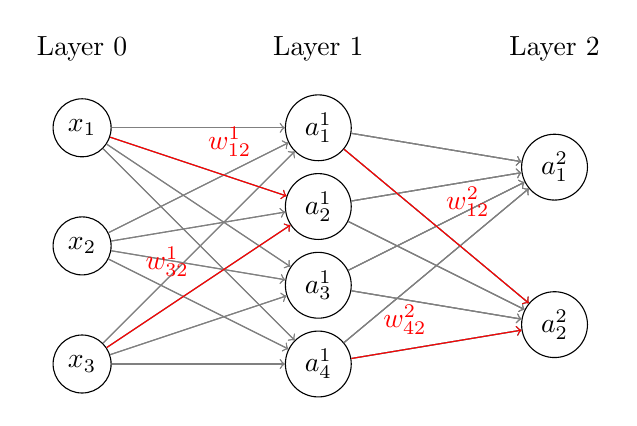
\begin{tikzpicture}
        % layer 0: input layer
        \begin{scope}[name prefix=layer0-]
            \node at (0, 0) {Layer 0};
            \node[circle, draw] (1) at (0, -1) {$x_1$};
            \node[circle, draw] (2) at (0, -2.5) {$x_2$};
            \node[circle, draw] (3) at (0, -4) {$x_3$};
        \end{scope}

        % layer 1
        \begin{scope}[name prefix=layer1-]
            \node at (3, 0) {Layer 1};
            \node[circle, draw] (1) at (3, -1) {$a^1_1$};
            \node[circle, draw] (2) at (3, -2) {$a^1_2$};
            \node[circle, draw] (3) at (3, -3) {$a^1_3$};
            \node[circle, draw] (4) at (3, -4) {$a^1_4$};
        \end{scope}

        % layer 2
        \begin{scope}[name prefix=layer2-]
            \node at (6, 0) {Layer 2};
            \node[circle, draw] (1) at (6, -1.5) {$a^2_1$};
            \node[circle, draw] (2) at (6, -3.5) {$a^2_2$};
        \end{scope}

        % weights
        \foreach \x in {1, 2, 3} {
            \foreach \y in {1, 2, 3, 4} {
                \foreach \z in {1, 2} {
                    \draw[gray, ->] (layer0-\x) -- (layer1-\y);
                    \draw[gray, ->] (layer1-\y) -- (layer2-\z);
                }
            }
        }
        \draw (layer0-1) edge[red, ->] node[auto] {$w^1_{12}$} (layer1-2);
        \draw (layer0-3) edge[red, ->] node[auto] {$w^1_{32}$} (layer1-2);
        \draw (layer1-1) edge[red, ->] node[auto] {$w^2_{12}$} (layer2-2);
        \draw (layer1-4) edge[red, ->] node[auto] {$w^2_{42}$} (layer2-2);
    \end{tikzpicture}
    \end{center}
    \caption{A 2 Layer Neuron Network}
\end{figure}

\section{Notations}
\begin{description}
    \item[$L$] output layer.
    \item[$n_l$] number of neurons in layer $l$. In particular, $n_0 = n$.
    \item[$w^l_{ij}$] weight from the $i$-th neuron in the layer $l-1$ to the $j$-th neuron in the layer $l$.
    \item[$b^l_j$] bias of the $j$-th neuron in layer $l$.
    \item[$a^l_j$] activation of the $j$-th neuron in layer $l$.
    \item[$z^l_j$] raw output of the $j$-th neuron in layer $l$.
    \item[$\sigma^l_j$] activation function of the $j$-th neuron in layer $l$.
    \item[$\V{W}^l$] weight matrix connecting layer $l-1$ to layer $l$, i.e. $(w^l_{ij})$, of dimension 
    $(n_{l-1},\ n_l)$.
    \item[$\V{b}^l$] bias vector of layer $l$, i.e. $(b^l_j)$, of dimension $(1, n_l)$.
    \item[$\V{z}^l$] raw output vector of layer $l$, of dimension $(1, n_l)$.
    \item[$\V{a}^l$] activation vector of layer $l$, of dimension $(1, n_l)$.
    \item[$\V{\sigma}^l$] vector of activation functions of layer $l$, of dimension $(1, n_l)$.
\end{description}

Some basic equations:

\begin{align}
    z^0_j &= a^0_j = x_j\\
    z^l_j &= \sum_k a^{l-1}_{k} w^l_{kj} + b^l_j\quad\forall~l\geq 1\\
    a^l_j &= \sigma^l_j(z^l_j)
\end{align}
The corresponding matrix forms are:

\begin{align}
    \V{z}^0 &= \V{a}^0 = \V{x} = (x_1, x_2, \ldots, x_{n})\\
    \V{z}^l &= \V{a}^{l-1} \V{W}^l + \V{b}^l\\
    \V{a}^l &= \V{\sigma}^l(\V{z}^l)
\end{align}

For a single input example \V{x}, the cost function $C$ should only directly depend on the output layer $L$,
for example $C$ is the square loss function:
\begin{equation}\label{nn_square_loss}
    C = \frac{1}{2} ||\V{a}^L - \V{y}||^2_2
\end{equation}
For a collection of examples, the cost function is the average cost on those examples:
\begin{equation}
    C = \frac{1}{m} \sum_{i=1}^m C(\V{x}^i)
\end{equation}

\section{Backpropagation}
First let's consider the case with a single input example. Let $\delta^l_j$ be the error in the $j$-th neuron
in the $l$-th layer, i.e.
\begin{equation}\label{delta_l_j}
    \delta^l_j = \pfrac{C}{z^l_j}
\end{equation}

For the output layer $L$, by definition we have:
\begin{align*}
    \delta^L_j &= \pfrac{C}{z^L_j}\\
               &= \sum_k \pfrac{C}{a^L_k} \pfrac{a^L_k}{z^L_j}\\
               &= \pfrac{C}{a^L_j} \pfrac{\sigma^L_j(z^L_j)}{z^L_j}\\
               &= \pfrac{C}{a^L_j}\cdot (\sigma^L_j)'(z^L_j)
\end{align*}
Let $\V{\delta}^l = {(\delta^l_j)}_{1 \times n_l}$, then the above equation can be written as:
\begin{equation}
    \V{\delta}^L = \nabla_{\V{a}^L}C \odot (\V{\sigma}^L)'(\V{z}^L)
\end{equation}
For example, when $C$ is the square loss~\eqref{nn_square_loss}, $\nabla_{\V{a}^L}C = \V{a}^L - \V{y}$.
\par
We can write $\V{\delta}^l$ in terms of $\V{\delta}^{l+1}$ as following:
\begin{align*}
    \delta^l_j &= \pfrac{C}{z^l_j}\\
               &= \sum_k \pfrac{C}{z^{l+1}_k} \pfrac{z^{l+1}_k}{z^l_j}\\
               &= \sum_k \delta^{l+1}_k \sum_r \pfrac{a^l_r}{z^l_j} w^{l+1}_{rk}\\
               &= \sum_k \delta^{l+1}_k (\sigma^l_j)'(z^l_j) w^{l+1}_{jk}\\
               &= {\left(\V{\delta}^{l+1} \T{(\V{W}^{l+1})}\right)}_{j} (\sigma^l_j)'(z^l_j)
\end{align*}
Its corresponding matrix form is:
\begin{equation}
    \V{\delta}^l = \left(\V{\delta}^{l+1} \T{(\V{W}^{l+1})}\right) \odot (\V{\sigma}^l)'(\V{z}^l)
\end{equation}

Now, let's compute \pfrac{C}{b^l_j}:
\begin{align*}
    \pfrac{C}{b^l_j} &= \sum_k \pfrac{C}{z^l_k} \pfrac{z^l_k}{b^l_j}\\
                     &= \sum_k \delta^l_k \pfrac{b^l_k}{b^l_j}\\
                     &= \delta^l_j
\end{align*}
In shorthand, it can be rewritten as:
\begin{equation}
    \pfrac{C}{\V{b}} = \V{\delta}
\end{equation}

Similarly, we can compute \pfrac{C}{w^l_{ij}}:
\begin{align*}
    \pfrac{C}{w^l_{ij}} &= \sum_k \pfrac{C}{z^l_k} \pfrac{z^l_k}{w^l_{ij}}\\
                        &= \sum_k \delta^l_k \sum_r \pfrac{(a^{l-1}_r w^l_{rk} + b^l_k)}{w^l_{ij}}\\
                        &= \sum_k \delta^l_k a^{l-1}_i \delta_{kj}\\
                        &= a^{l-1}_i \delta^l_j
\end{align*}
In shorthand, it can be rewritten as:
\begin{equation}
    \pfrac{C}{\V{W}} = \V{a}_{\text{in}}\V{\delta}_{\text{out}}
\end{equation}

For simplicity, let's assume that all the activation functions are the same, i.e. $\sigma^l_i = \sigma$, then 
we can write the pseudocode of backpropagation algorithm easily as the following:

\begin{algorithm}
    \caption{Backpropagation}\label{backpropagation}
    \begin{algorithmic}[1]
        \Require $\V{x} = (x_1, x_2, \ldots, x_n)$
        \For{$l = 1$ \algorithmicto $L$}
            \State Compute $\V{z}^l = \V{a}^{l-1} \V{W}^l + \V{b}^l$ and $\V{a}^l = \sigma(\V{z}^l)$.
        \EndFor
        \State Compute $\V{\delta}^l = \nabla_{\V{a}^L}C \odot \V{\sigma}'(\V{z}^L)$
        \Comment{$\nabla_{\V{a}^L}C = \V{a}^L - \V{y}$ if $C$ is square loss.}
        \For{$l=L-1$ \algorithmicto $1$}
            \State Compute $\V{\delta}^l = \left(\V{\delta}^{l+1} \T{(\V{W}^{l+1})}\right) \odot \sigma'(\V{z}^l)$
        \EndFor
        \Ensure $\pfrac{C}{w^l_{ij}} = a^{l-1}_i \delta^l_j$ and $\pfrac{C}{b^l_j} = \delta^l_j$.
    \end{algorithmic}
\end{algorithm}

We are now ready to do the vectorization. Let $\V{x}^i$ and $\V{y}^i$
be the $i$-th example and its output respectively, let
\begin{align*}
    \V{X} &= {(\V{x}^1; \ldots; \V{x}^m)}_{m \times n}\\
    \V{Y} &= {(\V{y}^1; \ldots; \V{y}^m)}_{m \times n_L}
\end{align*}
the input matrix. 
Let $\V{z}^{i, l}, \V{a}^{i, l}, \V{\delta}^{i, l}$ be the raw output, output, error vectors w.r.t.\ the
$i$-th example respectively. Let 
\begin{align*}
    \V{Z}^l &= {(\V{z}^{1, l}; \ldots; \V{z}^{m, l})}_{m \times n_l}\\
    \V{A}^l &= {(\V{a}^{1, l}; \ldots; \V{a}^{m, l})}_{m \times n_l}\\
    \V{\Delta}^l &= {(\V{\delta}^{1, l}; \ldots; \V{\delta}^{m, l})}_{m \times n_l}
\end{align*}
then we have:
\begin{align}
    \V{Z}^l &= \V{A}^{l-1} \V{W}^l + \V{b}^l\\
    \V{A}^l &= \sigma(\V{Z}^l)\\
    \V{\Delta}^L &= \nabla_{\V{A}^L}C \odot \sigma'(\V{Z}^L)\\
    \V{\Delta}^l &= \left(\V{\Delta}^{l+1} \T{(\V{W}^{l+1})}\right) \odot \sigma'(\V{Z}^l)
\end{align}
If $C = \frac{1}{m}\sum_{i=1}^m C(\V{x}^i)$, then
$$\pfrac{C}{b^l_j} = \operatorname{reduce\_mean}(\operatorname{col}_j(\V{\Delta}^l))$$
and
$$\pfrac{C}{w^l_{ij}} = \operatorname{reduce\_mean}(\operatorname{col}_i(\V{A}^{l-1}) \odot 
\operatorname{col}_j (\V{\Delta}^l))$$

\section{Cost Functions}


\section{Regularizations}
\subsection{$L^1$ and $L^2$ Regularizations}

\subsection{Dropout}

% ========Bayesian Classifier=========
\chapter{Bayesian}
\include{part_1/bayes/bayesian_classifier}

% ========Clustering=================
\chapter{Clustering}
\section{Clustering}


% ========Expectation Maximalization====
\chapter{Expectation Maximalization}
\include{part_1/em/EM}

% ========Ensemble Learning============
\chapter{Ensemble Learning}
\section{AdaBoost}
AdaBoost combines a family of binary classification base (weak) learners from an algorithm linearly to get a stronger (more
powerful) one. It takes advantage
of a former learner and use its output to force the latter learner to focus more on those data on which the
former learner performs poorly. In this way, it hopes to make the aggregate learner performs well on all
training data. Thus AdaBoost focus more on reducing the bias. 
% AdaBoost algorithm
\begin{algorithm}
    \caption{AdaBoost}\label{AdaBoost}
    \begin{algorithmic}[1]
        \Require training set $D = \{(\V{x}_1, y_1), \ldots, (\V{x}_m, y_m)\}$; base learner $\mathcal{L}$;
        training round $T$.
        \State $\mathcal{D}_1(\V{x}) = \frac{1}{m}$.\Comment{$\mathcal{D}$ is a distribution over the input 
        examples.}
        \For{$t = 1$ \algorithmicto $T$}
            \State $h_t = \mathcal{L}(D, \mathcal{D}_t)$;
            \State $\varepsilon_t = \p_{\V{x}\sim\mathcal{D}_t}(h_t(\V{x})\neq f(\V{x}))$;\Comment{
            $\varepsilon_t$ is the error rate of $h_t$ w.r.t $\mathcal{D}_t$.}
            \breakif{$\varepsilon_t > 0.5$}\Comment{Base learner must be above average.}
            \State $\alpha_t = \frac{1}{2}\ln{\frac{1 - \varepsilon_t}{\varepsilon_t}}$;\label{AdaBoost_alphat}
            \State $\mathcal{D}_{t + 1}(\V{x}) = \frac{\mathcal{D}_t(\V{x})\exp(-\alpha_t f(\V{x})h_t(\V{x}))}
            {Z_t}$.\Comment{$Z_t$ is the normalization constant.}\label{AdaBoost_distritution}
        \EndFor
        \Ensure $H(\V{x}) = \sign(\displaystyle\sum_{t = 1}^T \alpha_t h_t(\V{x}))$
    \end{algorithmic}
\end{algorithm}

%TODO: equivalent to 0/1 loss function.
Consider the exponential loss function
\begin{equation}
    L_{\exp}(H | \mathcal{D}) = \E_{\V{x}\sim\mathcal{D}}[e^{-f(\V{x})H(\V{x})}]
\end{equation}
We want to find a linear combination of base learners 
$$ H(\V{x}) = \sum_{t=1}^T \alpha_t h_t(\V{x})$$
that minimize it. Although it is difficult to find such $H$ as a whole, we can approach this problem step by
step. That is, we first find some $h_1$ and $\alpha_1$ \st $H_1 = \alpha_1 h_1$ minimize the exponential loss,
then we find some $h_2$ and $\alpha_2$ \st $H_2 = H_1 + \alpha_2 h_2$ minimize the exponential loss too. And
we carray on this process until $t = T$. Assume we have $H_{t-1}$ and want to find the next learner and its
weight, that is, we want to find $\alpha_t$ and $h_t$ \st $H_t = H_{t-1} + \alpha_t h_t$ minimize the 
exponential loss. Since
\begin{align*}
    L_{\exp}(H_t | \mathcal{D}) &= L_{\exp}(H_{t-1} + \alpha_t h_t | \mathcal{D})\\
    &= \E_{\V{x}\sim \mathcal{D}}[e^{-f(\V{x})H_{t-1}(\V{x})}\cdot e^{-f(\V{x})\alpha_t h_t(\V{x})}]\\
    &= C_{t-1} \E_{\V{x}\sim \mathcal{D}}[\frac{e^{-f(\V{x})H_{t-1}(\V{x})}}{C_{t-1}}
    e^{-f(\V{x})\alpha_t h_t(\V{x})}]\\
    &= C_{t-1} \E_{\V{x}\sim \mathcal{D}_t}[e^{-f(\V{x})\alpha_t h_t(\V{x})}]
\end{align*}
where $C_{t-1} = \E_{\V{x}\sim\mathcal{D}}[e^{-f(\V{x})H_{t-1}(\V{x})}]$ is a constant and 
$\mathcal{D}_t = \frac{e^{-f(\V{x})H_{t-1}(\V{x})}}{C_{t-1}} \mathcal{D}$ is a distribution, we have
\begin{align}
    L_{\exp}(H_t | \mathcal{D}) &= C_{t-1} \left\{e^{-\alpha_t} \p_{\V{x}\sim\mathcal{D}_t}(f(\V{x})=h_t(\V{x})) 
    + e^{\alpha_t}\p_{\V{x}\sim\mathcal{D}_t}(f(\V{x})\neq h_t(\V{x}))\right\}\nonumber\\
    &= C_{t-1} \{e^{-\alpha_t}(1 - \varepsilon_t) + e^{\alpha_t}\varepsilon_t\}\label{Ada_exp_loss_expansion}
\end{align}
where $\varepsilon_t$ is the error rate of $h_t$ w.r.t.\ the distribution $\mathcal{D}_t$. Hence 
$$\pfrac{ }{\alpha_t}L_{\exp}(H_t | \mathcal{D}) = 0$$
implies 
\begin{equation}\label{AdaBoost_weight}
    \alpha_t = \frac{1}{2}\ln(\frac{1-\varepsilon_t}{\varepsilon_t})
\end{equation}
which justifies the choice of $\alpha_t$ in line~\algref{AdaBoost}{AdaBoost_alphat}. Moreover, 
$$\mathcal{D}_t = \frac{e^{-f(\V{x})H_{t-1}(\V{x})}}{C_{t-1}} \mathcal{D}$$
implies
\begin{align}
\mathcal{D}_{t+1}(\V{x}) &= \frac{e^{-f(\V{x})\alpha_t h_t(\V{x})}C_{t-1}\mathcal{D}_t(\V{x})}{C_t}\nonumber\\
                         &= \frac{e^{-f(\V{x})\alpha_t h_t(\V{x})}\mathcal{D}_t(\V{x})}{Z_t}
\end{align}
which justifies the choice of $\mathcal{D}_t$ in line~\algref{AdaBoost}{AdaBoost_distritution}. If we plug
equation~\eqref{AdaBoost_weight} into~\eqref{Ada_exp_loss_expansion}, we get
$$L_{\exp}(H_t | \mathcal{D}) = 2C_{t-1}\cdot\sqrt{\varepsilon_t (1-\varepsilon_t)}$$
Since the performance of the base learner is slightly above the average, that is, 
$\varepsilon_t < \frac{1}{2}$, the minimum of the exponential loss is achieved at the $h_t$ which has 
the minimal error rate w.r.t.\ $\mathcal{D}_t$. That is, $h_t$ is the output of the algorithm w.r.t.\ the 
distribution $\mathcal{D}_t$ over the training data.


\section{Bagging}
Bagging is short for bootstrap aggregating, namely we use bootstrap sampling to sample $T$ groups of training
data, and train $T$ base learners using those groups, then we aggregate those $T$ base learners into one via 
plurality vote (for classification) or averaging (for regression). In this way, bagging mainly focus on
reducing the variance.

% Bagging algorithm
\begin{algorithm}
    \caption{Bagging}\label{Bagging}
    \begin{algorithmic}[1]
        \Require training set $D = \{(\V{x}_1, y_1), \dotsc, (\V{x}_m, y_m)\}$; base learner $\mathcal{L}$;
        training round $T$.
        \For{$t = 1$ \algorithmicto $T$}
            \State $h_t = \mathcal{L}(D, \mathcal{D}_{bs})$\Comment{bs stands for bootstrap sampling.} 
        \EndFor
        \Ensure $H(\V{x}) = \displaystyle\argmax_{y\in \mathcal{Y}}\sum_{t=1}^T 1(h_t(\V{x}) = y)$\Comment{$H$
        is the plurality vote of $h_t$.}
    \end{algorithmic}
\end{algorithm}

Unlike the AdaBoost in the preceding section, bagging can be applied to multiclass classification and
regression without any modifications. Morover, due to bootstrap sampling, we have around $36.8\%$ samples
untouched in each training, which can be used to do the out-of-bag estimation for testing the generalization
ability.

\section{Random Forest}
A forest is a collection of trees. When applying bagging to decision tree, we get a forest. A random forest is
obtained this way with randomness. Namely, when deciding the best feature for an internal node, we restrict 
the candidates to an randomly chosen subset from all possible features. Usually, the size of subset is 
$\log_2 d$ where $d$ is the total number of all possible features.

% 

% ========Dimension Reduction=========
\chapter{Dimension Reduction}
\section{Low-dimensional embedding}
Let the feature space $\mathcal{X} = \mathbb{R}^d$. Our goal is to find an embedding of all samples into a
low dimension space $\mathbb{R}^{d'}$, here $d' \leq d$. That is, we want to find a map $e: \mathbb{R}^d
\longrightarrow \mathbb{R}^{d'}$ \st for any samples $\V{x}_i, \V{x}_j$, we have 
$$\dist(e(\V{x}_i), e(\V{x}_j)) = \dist(\V{x}_i, \V{x}_j)$$
Thus ${\left\{e(\V{x}_i)\right\}}_i$ is a low-dimensional embedding of the original samples. 

Let $\V{D} = {\left(\dist(\V{x}_i, \V{x}_j)\right)}_{m \times m}$ be the distance matrix of the samples 
${\left\{\V{x}_i\right\}}_i$, we want to find the embedding matrix $\V{Z} \in \mathbb{R}^{m \times d'}$, \st 
$||\V{z}_i - \V{z}_j|| = \V{D}_{ij}$, where $\V{Z} = (\V{z}_1; \dotsc; \V{z}_m)$ and 
$\V{D}_{ij} = \dist(\V{x}_i, \V{x}_j)$. Hence we have 
$$ \V{D}_{ij}^2 = ||\V{z}_i||^2 + ||\V{z}_j||^2 - 2 \langle\V{z}_i, \V{z}_j\rangle$$
Let $\V{B} = {\left(b_{ij}\right)}_{m \times m}= \V{Z}\T{\V{Z}}$ where $b_{ij} = \langle\V{z}_i, \V{z}_j\rangle$, 
we have
\begin{equation}\label{DR_Dij}
    \V{D}_{ij}^2 = b_{ii} + b_{jj} - 2 b_{ij}
\end{equation}
Let $\V{c} = \frac{1}{m}\sum_i \V{z}_i$, then ${\left\{\V{z}_i - \V{c}\right\}}_i$ is an embedding with the
property that $\sum_i(\V{z}_i - \V{c}) = 0$. Hence we can require that $\sum_i \V{z}_i = 0$ in the above
discussion. Then from equation~\eqref{DR_Dij}, we know that:
\begin{align}
    \sum_i \V{D}_{ij}^2 &= \tr(\V{B}) + m b_{jj}\\
    \sum_j \V{D}_{ij}^2 &= \tr(\V{B}) + m b_{ii}\\
    \sum_{i,j} \V{D}_{ij}^2 &= 2m \tr(\V{B})
\end{align}
From the above equations, we have
\begin{equation}\label{DR_bij}
    b_{ij} = -\frac{1}{2}\left(\V{D}_{ij}^2 - \frac{1}{m}\sum_i \V{D}_{ij}^2 - \frac{1}{m} \sum_j \V{D}_{ij}^2
    + \frac{1}{m^2}\sum_{i,j}\V{D}_{ij}^2\right)
\end{equation}
That is, $\V{B}$ is totally determined by $\V{D}$. Let $\V{B} = \V{V}\V{\Lambda}\T{\V{V}}$ be the eigenvalue
decomposition of $\V{B}$. Since $\V{B}$ is semi-positive, $\V{\Lambda}$ is a diagonal matrix with non-negative
diagonals. Let $\V{\Lambda}_*$ be the diagonal matrix obtained by removing the zero eigenvalues from 
$\V{\Lambda}$ and $\V{V}_*$ the matrix by removing the corresponding columns of $\V{V}$. Then it's easy to 
conclude that 
$$\V{Z} = \V{V}_*\V{\Lambda}_*^{\nicefrac{1}{2}}$$
is what we want. Hence the dimension $d'$ is totally determined by the distance matrix $\V{D}$. 

In practise, we often fix some $d' \ll d$ at first, then obtain $\V{\Lambda}_*$ by keeping the $d'$ largest 
eigenvalues and remove the rest, and $\V{V}_*$ the corresponding matrix. By this way, we may lose some 
precision in keeping the pairwise distance, but we can greatly reduce the dimension.

\begin{algorithm}
    \caption{Multiple Dimensional Scaling}
    \begin{algorithmic}[1]
        \Require the distance matrix $\V{D}_{m \times m}$; dimension $d'$.
        \State Compute the matrix $\V{B}$ according to equation~\eqref{DR_bij}.
        \State Eigenvalue decomposition: $\V{B} = \V{V} \V{\Lambda}\T{\V{V}}$.
        \State Let $\V{\Lambda}_*$ be the diagonal matrix with the $d'$ largest eigenvalues and $\V{V}_*$ the
        matrix with the corresponding eigenvectors.
        \Ensure Low-dimensional embedding: $\V{Z} = {\left(\V{V}_* \V{\Lambda}_*^{\nicefrac{1}{2}}\right)}_{m 
        \times d'}$
    \end{algorithmic}
\end{algorithm}

\section{Linear Dimension Reduction}
The simplest way to reduce dimension is by dropping some coordinates, that is, via projection. This keeps the
linear structure of the samples. A more generalized way is via linear transformation: $A: \mathbb{R}^d 
\longrightarrow \mathbb{R}^{d'}$. In matrix form, we want to find a transformation matrix 
$\V{W} \in \mathbb{R}^{d \times d'}$ \st for any row vector $\V{x} \in \mathbb{R}^d$, we have
$A(\V{x}) = \V{x} \V{W}$. If we write $\V{W} = \left(\V{w}_1, \dotsc, \V{w}_{d'}\right)$, then we have
$A(\V{x}) = \left(\langle \V{x}, \V{w}_1\rangle, \dotsc, \langle \V{x}, \V{w}_{d'}\rangle\right)$. If
${\left\{\V{w}_i\right\}}_{i=1}^{d'}$ is orthonormal, then $A(\V{x})$ is the projection of $\V{x}$ into the
subspace spanned by ${\left\{\V{w}_i\right\}}_{i=1}^{d'}$. It's easy to see that if 
$\V{X} = {\left(\V{x}_1; \dotsc; \V{x}_m\right)}_{m \times d}$ is the feature matrix of the samples, then 
$\V{Z} = \V{X} \V{W} \in \mathbb{R}^{m \times d'}$ is the representation matrix desired.

\subsection{Principle Component Analysis}
The naive projection method may fail because of the huge possibility of dropping those components that really
matters while keeping those that have little information about the dataset. To overcome this, we need to
determine what is it mean for a component to be principle. A natrual measurement is the variance. Namely, 
the component with largest variance and lowest covariance w.r.t.\ others counts most. We only drop out those 
with small variances. 
\par
Let $\V{X} = {\left(\V{x}_1; \dotsc; \V{x}_m\right)}$ be the feature matrix as above. Without loss of 
generality, we may assume that $\sum_i \V{x}_i = 0$. Then $\T{\V{X}}\V{X} \in \mathbb{R}^{d \times d}$ is the
covariance matrix of $\V{X}$. If $\T{\V{X}}\V{X}$ is diagonal, then the largest eigenvalue corresponds to the 
principle component. Hence we may keep the components corresponding to the $d'$ largest eigenvalues. If 
$\T{\V{X}}\V{X}$ is not diagonal, let $\T{\V{X}}\V{X} = \V{V}\V{\Lambda}\T{\V{V}}$ be its eigenvalue 
decomposition. Then we have $\T{\V{V}}\T{\V{X}}\V{X}\V{V} = \V{\Lambda}$. The matrix 
${\left(\V{V}_*\right)}_{d \times d'}$ consists of the eigenvectors corresponding to the $d'$ largest 
eigenvalues of $\V{\Lambda}$ is the desired transformation matrix. And $\V{X}\V{V}_*$ is the representation of
the original samples in low dimensional space $\mathbb{R}^{d'}$.

% algorithm of PCA
\begin{algorithm}
    \caption{Principle Component Analysis}\label{algorithm:pca}
    \begin{algorithmic}[1]
        \Require dataset $D = \left\{\V{x}_1, \dotsc, \V{x}_m\right\}$; dimension $d'$.
        \State Compute the center of samples: $\V{c} = \frac{1}{m}\sum_i \V{x}_i$
        \State $\V{x}_i \gets \V{x}_i -\V{c}$
        \State Compute the covariance matrix $\T{\V{X}}\V{X}$\Comment{$\V{X}=(\V{x}_1; \dotsc;\V{x}_m)$}
        \State Eigenvalue decomposition: $\T{\V{X}}\V{X} = \V{V}\V{\Lambda}\T{\V{V}}$
        \State Fetch the (column) eigenvectors $\V{w}_1, \dotsc, \V{w}_{d'}$ from $\V{V}$ corresponding to the
        $d'$ largest eigenvalues of $\V{\Lambda}$.
        \Ensure transformation matrix $\V{W} = \left(\V{w}_1, \dotsc, \V{w}_{d'}\right)$
    \end{algorithmic}
\end{algorithm}

\begin{re}
    The PCA method actually consists of two steps:
    \begin{compactenum}
        \item Centralization: $\V{x} \gets \V{x} -\V{c}\quad\forall~\V{x}$ where the center $\V{c}$ is computed
        from the the given data set.
        \item Linear transformation: $\V{z} = \V{x} \V{W}$ where $\V{z}, \V{x}$ are both row vectors and
        $\V{z}$ is the desired representation in low dimensional space.
    \end{compactenum}
    Of course, those two steps should also apply to unseen data.
\end{re}

\begin{re}
    In the above PCA algorithm~\ref{algorithm:pca}, we can use the \textbf{singular value decomposition}
    instead of the eigenvalue decomposition. Let $\V{X} = \V{U}\V{\Sigma}\T{\V{V}}$ be the singular value 
    decomposition of $\V{X}$, then we have $\T{\V{X}}\V{X} = \V{V} \T{\V{\Sigma}}\V{\Sigma} \T{\V{V}}$. Notice
    that $\T{\V{\Sigma}}\V{\Sigma}$ is a diagonal. We can proceed as in the above algorithm to get the
    transformation matrix.
\end{re}

There are other approaches to derive the PCA algorithm.

% ========Computational Learning Theory
\chapter{Computational Learning Theory}
\section{Computational Learning Theory}
In this section, we mainly consider supervised learning.
Let $\mathcal{X}$ be the instance space, $\mathcal{Y}$ the label set, $D = \{(\V{x}_1, y_1), \ldots, 
(\V{x}_m, y_m)\}$ the training set. Assume $\mathcal{D}$ is the distribution on $\mathcal{X}$, and all 
instances of $D$ are sampled i.i.d.\ according to $\mathcal{D}$. Let \hypo{f} be the underlying labeling 
function and \hypo{h} any prediction function, then the \textbf{true (generalization) loss (error)} is defined
as:
$$L_{\mathcal{D}, f}(h) := \p_{\V{x}\sim\mathcal{X}}(h(\V{x})\neq f(\V{x})) := \mathcal{D}\left(\{\V{x}: h(\V{x})
\neq f(\V{x})\}\right)$$
the \textbf{empirical risk (error, loss)} is defined as:
$$L_S(h) = \frac{1}{m}\sum_{i=1}^m \indi(h(\V{x})\neq f(\V{x}))$$

\subsection{Probably Approximately Correct Learning}

% concept class.
\begin{df}[Concept class]
    A (target) concept is just a true labeling function \hypo{c}, that is, for any instace $(\V{x}, y)$ 
    (assuming sampling process is noise free) we have $c(\V{x}) = y$. The collection $\mathcal{C}$ of all 
    target concepts is called the concept class.
\end{df}

% hypothesis space.
\begin{df}[Hypothesis space]
    The collection of all labeling functions \hypo{f} a learner $\mathcal{L}$ can return is called the 
    hypothesis space (w.r.t.\ $\mathcal{L}$). We denote it as $\mathcal{H}$.
\end{df}

% inductive bias.
\begin{re}[Inductive bias]
    By restricting our learner to the hypothesis space instead of arbitrary predictors, we bias it toward a 
    particular set of predictors. Such restrictions are called \textbf{inductive bias}.
\end{re}

% realizability assumption.
\begin{df}[Realizability Assumption]
    The realizable assumption asserts that there is a $h^* \in \mathcal{H}$ s.t.\ 
    $L_{\mathcal{D}, f}(h^*) = 0$.
\end{df}

\begin{re}
    The realizable assumption implies that with probability 1 over i.i.d.\ samples $D$, we have $L_D(h^*) = 0$.
    That is, $\mathcal{D}^m(\{D: L_D(h^*) = 0\}) = 1$.
\end{re}

% PAC learnability.
\begin{df}[PAC learnability]\label{PAC_learnability}
    The concept class $\mathcal{C}$ is PAC learnable w.r.t.\ a hypothesis space $\mathcal{H}$ if there exist
    \begin{enumerate}
        \item a function $m: {(0, 1)}^2 \longrightarrow \mathbb{N}$;
        \item a learner $\mathcal{L}$.
    \end{enumerate}
    s.t.\ for any $\varepsilon, \delta \in (0, 1)$, for any distribution $\mathcal{D}$ over $\mathcal{X}$, and
    for any concept \hypo{c}, if the realizable assumption holds w.r.t.\ $\mathcal{H}, \mathcal{D}, c$, then
    when applying the learner $\mathcal{L}$ to $m \geq m(\varepsilon, \delta)$ i.i.d.\ samples generated by
    $\mathcal{D}$ and labeled by $c$, the learner returns a hypothesis $h$ s.t.\ with probability at least 
    $1 - \delta$ (over the choice of the samples), we have $L_{\mathcal{D},c}(h) \leq \varepsilon$. That is,
    $$\mathcal{D}^m(\{D: L_{\mathcal{D},c}(h) \leq \varepsilon\}) \geq 1 - \delta$$
\end{df}

% sample complexity.
\begin{df}[Sample complexity]
    The sample complexity of a learner is the minimal number of examples needed for the learner to produce a 
    PAC solution on any i.i.d.\ data sets with that many samples. That is, it is the minimum of all 
    $m(\varepsilon, \delta)$ where $m$ satisfies the requirements in definition~\ref{PAC_learnability}.
\end{df}

% agnostic PAC learnability.

% ========Reinforcement Learning
\chapter{Reinforcement Learning}
Let $X$ be the state space, $A$ the action space. Reinforcement learning can be described as a
\textbf{Markov Decision Process}: system changes from a state to another under the actions from $A$ with a 
rewarding function grading the change. That is, a reinforcement learning is a quadruple $E = \langle X, A, P,
R\rangle$, where $P: X \times A \times X \longrightarrow \mathbb{R}$ describes the probability of a state
changed into another via an action from $A$ and $R: X \times A \times X \longrightarrow \mathbb{R}$ describes
the reward of that change. Sometimes the rewarding function only depends on states, that is $R: X \times X
\longrightarrow \mathbb{R}$. Note that given a state $x$ and an action $a$ that can act on it, the resulting 
state $x'$ may not be unique, but the identity $\sum_{x'\in X}P_{x\rightarrow x'}^a = 1$ always holds true.
\par
The goal of reinforcement leanring is to find a \hl{policy $\pi$} dictating which action to take given a state
$x$. $\pi$ can be described in a determinate form $\pi: X \longrightarrow A$, which dictates that action
$\pi(x)$ must be performed on state $x$. It can also be described in a probability form: $\pi: X \times A
\longrightarrow \mathbb{R}$ where $\pi(x, a)$ is the probability of performing action $a$ on $x$. Obviously,
the determinate form is a special case of the probability form. The performance measurement of the policy is 
the accumulated reward gained from performing this policy for a reasonably long time. The \textbf{$T$ steps
accumulated reward} $\E[\frac{1}{T}\sum_{t=1}^{T}r_t]$ and \textbf{$\gamma$ discount accumulated reward}
$\E[\sum_{t=0}^{\infty}\gamma^t r_{t+1}]$ are two commonly used accumulated rewards, where $r_t$ is the reward
of step $t$.

\section{K-armed Bandit}
The K-armed bandit is a model of one step reinforcement learning. Every time you pull one arm of the machine,
it gives you some rewards with certain probability. The goal is to acquire as many rewards as possible.

\subsection{Exploration and Exploitation}
The \textbf{exploration-only} method tries to figure out the expectation reward of each arm. It divides the 
exploration chance evenly on each arm, and use the average reward of each arm as the expectation reward. This
method may do a good job in estimating each arm's reward, but it may miss the opportunity to get the most 
rewards. The \textbf{exploitation-only} method, on the other hand, only pulls the arm that gives the most 
average rewards so far. Since it dosen't care about the expectation reward of each arm, it may also miss the
opportunity to get the most rewards. 

\subsection{$\varepsilon$-greedy}
The $\varepsilon$-greedy is a compromise between exploration-only and exploitation-only method. At
each try, it performs exploration-only method with a probability $\varepsilon$ and exploitation-only method
the other $1 - \varepsilon$.\par
Let $Q_n(k)$ denote the average reward of arm $k$ with $n$ tries and $v_n^k$ its n-th reward, then it is 
clearly that
$$Q_n(k) = \frac{1}{n} ((n-1)Q_{n-1}(k) + v_n^k)$$
This is the updating rules for the average reward.

% epsilon-greedy algorithm
\begin{algorithm}
    \caption{$\varepsilon$-greedy}\label{epsilon_greedy_for_K_arm_bandit}
    \begin{algorithmic}[1]
        \Require number of arms $K$; rewarding function $R$; number of tries $T$; exploration threshold 
        $\varepsilon$.
        \State $r = 0$\Comment{the accumulated reward.}
        \State $Q(i) = 0, \quad count(i) = 0 \quad \forall~i=1,\ldots,K$\Comment{Initialization.}
        \For{$t = 1$ \algorithmicto $T$}
            \If{$rand() < \varepsilon$}
                \State $k = rand(\{1, \ldots, K\})$\Comment{choose with equal probability}
            \Else
                \State $k = \argmax_i Q(i)$
            \EndIf
            \State $v = R(k)$
            \State $r \gets r + v$
            \State $Q(k) \gets \frac{count(k) \cdot Q(k) + v}{count(k) + 1}$
            \State $count(k) \gets count(k) + 1$
        \EndFor
        \Ensure the accumulated reward $r$.
    \end{algorithmic}
\end{algorithm}

% TODO: analysis of the epsilon-greedy.

\subsection{Softmax}
Softmax algorithm is another way of compromising between the exploration-only and exploitation-only methods. 
Unlike the $\varepsilon$-greedy algorithm which uses a threshold to determine how to choose an arm, softmax 
attach each arm with a probability to be chosen base on its current average reward. The probability 
distribution among the arms is a Boltzmann distribution, namely:
\begin{equation}\label{K_arm_bandit_softmax}
P(k) = \frac{e^{\frac{Q(k)}{\tau}}}{\sum_{i=1}^K e^{\frac{Q(i)}{\tau}}}\quad\forall~k = 1,\ldots,K
\end{equation}
where the parameter $\tau > 0$. Apparently, if $\tau$ is close to $0$, the softmax favours the arm with
the highest average reward, which is the case of exploitation-only method; if $\tau$ is very large (close to 
$+\infty$), the softmax degenerates to uniform distribution, which is the case of exploration-only method.

% softmax algorithm for K-arm bandit.
\begin{algorithm}
    \caption{Softmax}\label{Softmax_for_K_arm_bandit}
    \begin{algorithmic}[1]
        \Require number of arms $K$; rewarding function $R$; number of tries $T$; parameter $\tau$.
        \State $r = 0$
        \State $Q(i) = 0, \quad count(i) = 0\quad\forall~i=1,\ldots, K$
        \For{$t = 1$ \algorithmicto $T$}
            \State choose $k$ according to the distribution given by equation~\eqref{K_arm_bandit_softmax}.
            \State $v = R(k)$
            \State $r \gets r + v$
            \State $Q(k) \gets \frac{count(k)\cdot Q(k)}{count(k) + 1}$
            \State $count(k) \gets count(k) + 1$
        \EndFor
        \Ensure the accumulated reward $r$.
    \end{algorithmic}
\end{algorithm}

% TODO: analysis of the softmax algorithm.

\newpage
\section{Model-based Learning}
In model-based learning, the quadruple $E = \langle X, A, P, R\rangle$ are known to us. That is, we know all
the possible states, all the possible actions that may act on them, the transition function which describes
the probability of one state changing into another under some action, the rewarding function which grades the
change. In the following discussion, we assume that \magenta{the state space $X$ and the action space $A$ are
finite}.

\subsection{Policy Measurement}
Let $V^\pi(x)$ be the expected reward gained from applying policy $\pi$ on the starting state $x$, 
$Q^\pi(x, a)$ the expected reward gained from first applying action $a$ then policy $\pi$ on the starting
state $x$. $V$ and $Q$ are called \textbf{state value function} and \textbf{state-action value function}
respectively. \par
By definition, we can write the state value function as:
\begin{align}
    V^\pi_T(x) &= \E_\pi\left[\frac{1}{T}\sum_{t=1}^{T}r_t | x_0 = x\right], &\text{$T$ steps}
    \label{state_value_T}\\
    V^\pi_\gamma(x) &= \E_\pi\left[\sum_{t=0}^{\infty} \gamma^t r_{t+1} | x_0 = x\right], &\text{$\gamma$ 
    discount}\label{state_value_gamma}
\end{align}
Similarly, we can write the state-action value function as:
\begin{align}
    Q^\pi_T(x, a) &= \E_\pi\left[\frac{1}{T}\sum_{t=1}^T r_t | x_0 = x, a_0 = a\right], &\text{$T$ steps}
    \label{state-action_value_T}\\
    Q^\pi_\gamma(x, a) &= \E_\pi\left[\sum_{t=0}^\infty \gamma^t r_{t+1} | x_0 = x, a_0 = a\right] &\text{
    $\gamma$ discount}\label{state-action_value_gamma}
\end{align}
\par
Since the next state of the system only depends on the current state, those value functions can be written in
a recursive form. For example, the $T$ steps accumulated state value function~\eqref{state_value_T} can be 
written as:
\begin{align}
    V^\pi_T(x) &= \E_\pi \left[\frac{1}{T}\sum_{t=1}^T r_t | x_0 = x\right]\nonumber\\
               &= \E_\pi \left[\frac{1}{T} r_1 + \frac{T-1}{T}\frac{1}{T-1}\sum_{t=2}^T r_t | x_0 = x\right]
               \nonumber\\
               &= \sum_{a\in A}\pi(x, a)\sum_{x'\in X}P_{x\rightarrow x'}^a\left(\frac{1}{T}
               R_{x\rightarrow x'}^a + \frac{T-1}{T}\E_\pi\left[\frac{1}{T-1}\sum_{t=1}^{T-1}r_t | x_0=x'
               \right]\right)\nonumber\\
               &= \sum_{a\in A}\pi(x, a)\sum_{x'\in X}P_{x\rightarrow x'}^a\left(\frac{1}{T}
               R_{x\rightarrow x'}^a + \frac{T-1}{T} V^\pi_{T-1}(x')\right)\label{state_value_T_expansion}
\end{align}

% algorithm for calculating T steps accumulated state value function.
\begin{algorithm}
    \caption{$T$ steps accumulated state value function}
    \begin{algorithmic}[1]
        \Require $E = \langle X, A, P, R\rangle$; policy $\pi$; steps $T$.
        \State $V(x) = 0\quad\forall~x\in X$
        \For{$t=1$ \algorithmicto $T$}
            \State $\displaystyle V'(x) = \sum_{a\in A}\pi(x,a)\sum_{x'\in X}P_{x\rightarrow x'}^a 
            \left(\frac{1}{t} R_{x\rightarrow x'}^a + \frac{t-1}{t}V(x')\right)\quad\forall~x\in X$
            \If{$t = T+1$}
                \State \algorithmicbreak
            \Else
                \State $V \gets V'$
            \EndIf
        \EndFor
        \Ensure state value function $V$.
    \end{algorithmic}
\end{algorithm}

Similarly, the $\gamma$ discount accumulated state value function~\eqref{state_value_gamma} can be written as:
\begin{align}
    V^\pi_\gamma(x) &= \E_\pi\left[\sum_{t=0}^\infty \gamma^t r_{t+1} | x_0 = x\right]\nonumber\\
                    &= \E_\pi\left[r_0 + \gamma \sum_{t=1}^\infty \gamma^{t-1}r_{t+1} | x_0=x\right]\nonumber\\
                    &= \sum_{a\in A}\pi(x, a)\sum_{x'\in X}P_{x\rightarrow x'}^a \left(R_{x\rightarrow x'}^a + 
                    \gamma \E_\pi\left[\sum_{t=0}^\infty \gamma^t r_{t+1} | x_0 = x'\right]\right)\nonumber\\
                    &= \sum_{a\in A}\pi(x, a)\sum_{x'\in X}P_{x\rightarrow x'}^a \left(R_{x\rightarrow x'}^a +
                    \gamma V^\pi_\gamma(x')\right)\label{state_value_gamma_expansion}
\end{align}

% algorithm for gamma discount accumulated state value function.
\begin{algorithm}
    \caption{$\gamma$ discount accumulated state value function}
    \begin{algorithmic}[1]
        \Require $E = \langle X, A, P, R\rangle$; policy $\pi$; parameter $\gamma$; threshold $\theta$.
        \State $V(x) = 0\quad\forall~x\in X$
        \Loop
            \State $\displaystyle V'(x) = \sum_{a\in A}\pi(x,a)\sum_{x'\in X}P_{x\rightarrow x'}^a 
            \left(R_{x\rightarrow x'}^a + \gamma V(x')\right)\quad\forall~x\in X$
            \If{$\displaystyle\max_{x\in X}|V(x) - V'(x)| < \theta$}
                \State \algorithmicbreak
            \Else
                \State $V \gets V'$
            \EndIf
        \EndLoop
        \Ensure state value function $V$.
    \end{algorithmic}
\end{algorithm}

% formulas for state-action value functions.
Since the state-action value functions are just the state value functions with the given first action, we can 
easily write the state-action value functions in terms of state value functions:
\begin{align}
    Q^\pi_T(x, a) &= \sum_{x' \in X} P_{x \rightarrow x'}^a\left(\frac{1}{T}R_{x \rightarrow x'}^a +
    \frac{T-1}{T}V^\pi_{T-1}(x')\right)\label{state-action_value_T_expansion}\\
    Q^\pi_\gamma(x, a) &= \sum_{x' \in X} P_{x \rightarrow x'}^a\left(R_{x \rightarrow x'}^a + \gamma 
    V^\pi_\gamma(x')\right)\label{state-action_value_gamma_expansion}
\end{align}
Hence it is obvious that:
\begin{equation}\label{relation_V_Q}
V^\pi(x) = \sum_{a \in A}\pi(x, a)Q^\pi(x, a)
\end{equation}

% TODO: algorithms for state-action value functions.

\subsection{Policy Improvement}
Of course, the best policy is the one that maximize the state value function, i.e.
$$\pi^* = \argmax_\pi \sum_{x \in X}V(x)$$
Due to the recursive nature of the state value functions~\eqref{state_value_T_expansion}
and~\eqref{state_value_gamma_expansion}, we can conclude that if there is no restriction on the policies that 
we can choose, the optimal state value functions satisfy the following equations:
\begin{align}
    V^*_T(x) &= \max_{a \in A} \sum_{x' \in X}P_{x \rightarrow x'}^a\left(\frac{1}{T}R_{x \rightarrow x'}^a +
    \frac{T-1}{T}V^*_{T-1}(x')\right)\\
    V^*_\gamma(x) &= \max_{a \in A} \sum_{x' \in X}P_{x \rightarrow x'}^a\left(R_{x \rightarrow x'}^a + \gamma
    V^*_\gamma(x')\right)
\end{align}
That is,
\begin{equation}\label{relation_optimal_V_Q}
    V^*(x) = \max_{a \in A}Q^*(x, a)
\end{equation}
This in turn gives us the expression of $Q^*(x, a)$:
\begin{align}
    Q^*_T(x, a) &= \sum_{x' \in X} P_{x \rightarrow x'}^a\left(\frac{1}{T}R_{x \rightarrow x'}^a +
    \frac{T-1}{T}\max_{a' \in A}Q^*_{T-1}(x',a')\right)\\
    Q^*_\gamma(x, a) &= \sum_{x' \in X} P_{x \rightarrow x'}^a\left(R_{x \rightarrow x'}^a + \gamma 
    \max_{a' \in A}Q^*_\gamma(x', a')\right)
\end{align}

The relation between optimal state value function and optimal state-action value 
function~\eqref{relation_optimal_V_Q} shed light on how to improve the current policy: \magenta{always choose 
the current best action for the state}. That is, let 
\begin{equation}
\pi'(x) = \argmax_{a \in A}Q^\pi(x, a)\quad\forall~x \in X
\end{equation}
Then by relation~\eqref{relation_V_Q}, we have
$$Q^\pi(x, \pi'(x)) \geqslant V^\pi(x)$$
Since $\pi'(x)$ is the action that should be taken on the state $x$, by relation~\eqref{relation_V_Q} again, 
we have
\begin{align*}
    V^{\pi'}(x) &= \sum_{a \in A}\pi'(x, a) Q^{\pi'}(x, a)\\
              &= Q^{\pi'}(x, \pi'(x))
\end{align*}
This gives us the following estimate:
\begin{align*}
    V^\pi(x) - V^{\pi'}(x) &\leqslant Q^\pi(x, \pi'(x)) - Q^{\pi'}(x, \pi'(x))\\
                           &\leqslant \sum_{x' \in X}P_{x \rightarrow x'}^{\pi'(x)}\cdot\gamma\left(V^\pi(x') - 
                           V^{\pi'}(x')\right)\\
                           &\leqslant \gamma \max_{x' \in X}\left(V^\pi(x') - V^{\pi'}(x')\right)\sum_{x' \in X}
                           P_{x \rightarrow x'}^{\pi'(x)}\\
                           &\leqslant \gamma \max_{x' \in X}\left(V^\pi(x') - V^{\pi'}(x')\right)
\end{align*}
Here, we use the fact that $P \geq 0$ and $\sum_{x' \in X}P_{x \rightarrow x'}^{\pi'(x)} = 1$. Since
$\gamma \in (0, 1)$, we conclude that
$$\max_{x \in X}\left(V^\pi(x) - V^{\pi'}(x)\right) \leqslant 0$$
That is 
$$V^\pi(x) \leqslant V^{\pi'}(x)\quad\forall~x \in X$$
This justifies the choice of $\pi'(x)$.
\begin{re}
    Note that the above discussion is also valid in the case of $T$-steps accumulated state value function
    with almost the same argument.
\end{re}

% TODO: policy iteration

% TODO: value iteration

\section{Model-free Learning}

% ===========Part Two: Papers=====================
\part{Selected Papers}

\chapter{Neuron Networks}
\section{Multilayer Feedforward Networks are Universal Approximators}


\end{document}